\documentclass[ejs]{imsart}

\RequirePackage[OT1]{fontenc}
\RequirePackage{amsthm,amsmath}
\RequirePackage[numbers]{natbib}
\RequirePackage[colorlinks,citecolor=blue,urlcolor=blue]{hyperref}

% settings
\pubyear{2019}
\volume{0}
\issue{0}
\firstpage{1}
\lastpage{8}

% add packages
\usepackage{enumitem}
\usepackage{amsfonts,graphicx,bbm}
%\usepackage[square,numbers]{natbib}
%\bibliographystyle{plain}
\usepackage{array,booktabs}
%\usepackage[margin=1.25in]{geometry}

%
% My definitions:
%
\def\bbN{{\mathbb N}}
\def\bbZ{{\mathbb Z}}
\def\bbR{{\mathbb R}}
\def\bbC{{\mathbb C}}

\def\P{{\mathbb P}}
\def\E{{\mathbb E}}

\newcommand{\var}{{\rm {Var}}}
\newcommand{\cov}{{\rm {Cov}}}

\def\N{\mathbb N}
\def\R{\mathbb R}
\def\Z{\mathbb Z}
\usepackage{bm}
\renewcommand\vec[1]{{\bm #1}}

\def\alert#1{\fbox{#1}}
\def\what{\widehat}
\def\noi{\noindent}
\def\MSE{{\rm m.s.e.}}
\newcommand\comment[1]{{}}
\def\refeq#1{(\ref{e:#1})}

\DeclareMathOperator*{\argmax}{arg\,max}
\DeclareMathOperator*{\argmin}{arg\,min}

\newcommand*\diff{\mathop{}\!\mathrm{d}}
\newcommand*\Diff[1]{\mathop{}\!\mathrm{d^#1}}
\newcommand\version[2]{{#1}} % The short version of the paper
%\newcommand\version[2]{{#2}} % The long version of the paper

%\startlocaldefs
\numberwithin{equation}{section}
\theoremstyle{plain}
\newtheorem{theorem}{Theorem}[section]
% my defs
\newtheorem{proposition}{Proposition}[section]
\newtheorem{definition}{Definition}[section]
\newtheorem{lemma}{Lemma}[section]
\newtheorem{corollary}{Corollary}[section]
\newtheorem{assumption}{Assumption}
\theoremstyle{remark}
\newtheorem{remark}{Remark}[section]
\newtheorem{example}{Example}[section]
%\endlocaldefs



\begin{document}

\begin{frontmatter}
\title{Multiple Testing for Categorical Data}%\thanksref{T1}}
\runtitle{Multiple Testing for Categorical Data}
%\thankstext{T1}{Footnote to the title with the `thankstext' command.}

\begin{aug}
\author{\fnms{Zheng} \snm{Gao}\thanksref{t1}\ead[label=e1]{gaozheng@umich.edu}}
%\and
%\author{\fnms{Second} \snm{Author}}%\thanksref{t3}\ead[label=e2]{second@somewhere.com}}

\address{Department of Statistics, University of Michigan, Ann Arbor, USA\\
\printead{e1}}

\thankstext{t1}{This research is supported by NSF Grant DMS-1830293, Algorithms for Threat Detection.}
%\thankstext{t2}{First supporter of the project}
%\thankstext{t3}{Second supporter of the project}
\runauthor{Z. Gao}

\affiliation{University of Michigan}

\end{aug}

\begin{abstract}
We study the high-dimensional multiple testing problems in categorical covariate screenings, where test statistics have approximately independent chi-square distributions.
In particular, we characterize two new phase transition phenomena, by deriving the statistical signal sizes necessary and sufficient for statistical procedures to 1) approximately, and 2) exactly select the set of relevant features in large dimensions.
Remarkably, the degrees-of-freedom parameter is irrelevant for the boundaries of both phase transitions.
Several well-known procedures are shown to attain these boundaries.

We then elucidate on the nature of statistical signal sizes in the context of association tests on contingency tables, typified by genome-wide association studies (GWAS). 
Specifically, we characterize the relationship between statistical signal size and marginal frequencies, odds ratio, and sample sizes. % in common association tests for binary traits.
% Specifically, detection of rare genetic variants associated with the outcomes requires more samples compared to common variants. 
% Specifically, the difficulty in detecting associations between genetic variants and phenotype traits is quantified in terms of the statistical signal sizes.
We further demonstrate, perhaps surprisingly, that balanced designs in case-control studies may \emph{not} deliver the highest power. % for detecting rare genetic variants with high odds ratios.
% Specifically, the amount of signal per sample is inherently smaller when rare variants are present. 
% In other words, 
% Further, case prevalence in the recruited subjects plays a role, while case prevalence in the population is irrelevant.

We provide explicit formulas for power calculations, as well as software tools for finding the optimal study designs.
These results allow us to perform power analysis for high-dimensional screening problems for categorical covariates, such as GWAS.
\end{abstract}

\begin{keyword}[class=MSC]
%\kwd[Primary ]{62G10, 62G20}
\kwd{62G10, 62G20}
%\kwd[; secondary ]{60K35}
\end{keyword}

\begin{keyword}
\kwd{Multiple testing}
\kwd{asymptotic optimality}
\kwd{family-wise error rate (FWER) control}
\kwd{false discovery rate (FDR) control}
\kwd{categorical data analysis}
\kwd{association tests}
\end{keyword}
\tableofcontents
\end{frontmatter}

\section{Introduction}
\label{sec:intro}

Multiple testing arises in a wide array of applied settings, ranging from anomaly
detection in sensor arrays to the selection of genes that are differentially expressed. 
This is particularly true in so-called discovery science, where the scientist proceeds by formulating hypotheses, testing each one of them on data, and following up on the most promising ones. 
Each step along the way is fraught with pitfalls, and even if the experiment was correctly designed and carried out, the scientist still needs to contend with the multitude of tests that were performed.

We are motivated by high-dimensional screening problems for categorical covariates.

A prototypical example is genome-wide association studies (GWAS).

\subsection{Genome-wide association studies}
\label{subsec:motivation-chisq}

Broadly speaking, genome-wide association studies aim to discover genetic variations that are linked to traits or diseases of interested, by testing for associations between genetic compositions of subjects and their phenotypes.
For example, in a typical GWAS for qualitative traits with a case-control design, a total of $n$ subjects are recruited consisting of $n_1$ subjects possessing the defined trait, and $n_2$ subjects without the trait.
The genetic compositions of these subjects are then sequenced for variations known as single-nucleotide polymorphisms (SNPs) at an array of $p$ genomic marker locations, and compared between the case group and the control group.

Focusing on one particular genomic location, the counts of observed genotypes, if two variants are present, can be tabulated as follows.
\begin{center}
    \begin{tabular}{cccc}
    \hline
    & \multicolumn{2}{c}{Genotype} & \\
    \cline{2-3}
    \# Observations & Variant 1 & Variant 2 & Total by phenotype \\
    \hline
    Cases & $O_{11}$ & $O_{12}$ & $n_1$ \\
    Controls & $O_{21}$ & $O_{22}$ & $n_2$ \\
    \hline
    \end{tabular}
\end{center}
To detect associations between the genotypes and the phenotypes, statistical tests are performed on the tabulated counts.
A common test of association is Pearson's Chi-square test, with statistic
\begin{equation} \label{eq:chisq-statistic}
    x = \sum_{j=1}^2 \sum_{k=1}^2 \frac{(O_{jk} - E_{jk})^2}{E_{jk}},
\end{equation}
where $E_{jk}$'s are the expected number of observations in respective cells, estimated empirically with $E_{jk} = (O_{j1}+O_{j2})(O_{1k}+O_{2k})/n$.
%E_{jk} = \Big(\sum_{l}O_{jl}\Big)\Big(\sum_{l}O_{lk}\Big)\Big/n.

Under the mild assumption that the counts $O_{jk}$'s follow a multinomial distribution, the statistic $x$ in \eqref{eq:chisq-statistic} can be shown to have an approximate $\chi^2(\lambda)$ distribution with $\nu=1$ degree of freedom at large sample sizes. 
When genotypes and phenotypes are independent, we have a non-centrality parameter $\lambda=0$; if dependence exists, we have $\lambda\neq0$ and its value depends on the underlying multinomial probabilities.
More generally, if we have a $J$ outcomes and $K$ genetic variants, assuming a $J\times K$ multinomial distribution, the statistic will follow approximately a $\chi^2_{\nu}(\lambda)$ distribution with $\nu = (J-1)(K-1)$ degrees of freedom for large sample sizes.

The same asymptotic distributional approximations are also applies to the likelihood ratio statistic, and many others under slightly different modeling assumptions \cite{gao2019upass}.
These association tests are performed at each of the $p$ SNP marker locations throughout the whole genome, yielding $p$ statistics having approximately (non)central $\chi^2_{\nu}$ distributions,
\begin{equation} \label{eq:model-chisquare-approx}
    x(i) \mathrel{\dot\sim} \chi_{\nu(i)}^2\left(\lambda(i)\right), \quad i=1,\ldots,p.
\end{equation}
Here $\lambda = (\lambda(i))_{i=1}^p$ is the $p$-dimensional non-centrality parameter, with $\lambda(i)=0$ indicating independence of the $i$-th SNP with the outcomes, and $\lambda(i)\neq0$ indicating associations.
Since dependence among the genetic markers at different locations (known as linkage disequilibrium in the genetics literature) decay rapidly as a function of the physical distance between them on the genome, the correlations of the resulting statistics also decay rapidly, resulting in statistics that are roughly independent except in very short ranges.

In genetic association studies where the number of genomic locations $p$ are in the order of $10^5$ or even $10^6$, it is often assumed that $\lambda$ is sparse, or approximately sparse.
That is, it is believed that only a small set of genetic variants have large influences on the outcome of the disease or trait of interest.
Under the stylized assumption of exact sparsity, $\lambda$ is assumed to have $s$ non-zero components, where $s$ is much smaller than the problem dimension $p$. 
The goal of researchers is usually two-fold: 1) to test if $\lambda(i)=0$ for all $i$, and 2) to estimate the set $S=\{i:\lambda(i)\neq 0\}$.
In other words, we look to determine if there are any genetic variation associated with the disease; and if there are associations, we wish to locate the associated variants.

The latter, referred to as the \emph{support recovery problem}, is the focus of this work.
We will study in detail the theoretical limits in support recovery problems in an idealized model where the statistics follow independent chi-square distributions,
\begin{equation} \label{eq:model-chisq}
    %x(i) \distras{\mathrm{ind.}} \chi_\nu^2\left(\lambda(i)\right), \quad i=1,\ldots,p.
    x(i) \sim \chi_\nu^2\left(\lambda(i)\right), \quad i=1,\ldots,p.
\end{equation}
We will also look for practical procedures that attain the performance limits, as soon as the problems become theoretically feasible.

\subsection{Two-sided alternatives of additive error models}
\label{subsec:motivation-additive}

Model \eqref{eq:model-chisq} also plays an important role in analyzing two-sided tests for additive error models,
\begin{equation} \label{eq:model-additive}
    x(i) = \mu(i) + \epsilon(i), \quad i=1,\ldots,p,
\end{equation}
where the errors $\epsilon$ are assumed to have standard normal distributions.
Under two-sided alternatives, unbiased tests call for rejecting the hypothesis $\mu(i)=0$ at locations where observations have large absolute values, or equivalently, large $x^2(i)$'s.
Taking squares on both sides of \eqref{eq:model-additive}, we arrive at Model \eqref{eq:model-chisq} with non-centrality parameters $\lambda(i) = \mu^2(i)$, and degrees-of-freedom parameter $\nu =1$.

The support recovery problem, in this case, is to locate the set of observations with mean shifts, $S=\{i:\mu(i)\neq 0\}$, where the mean shifts could take place in both directions.

While additive error models \eqref{eq:model-additive} have been studied extensively under one-sided alternatives (see, e.g., \cite{arias2017distribution, butucea2018variable, gao2018fundamental}), two-sided alternatives have been largely neglected.
It is not clear if there are simple equivalences of these two types of alternatives in support recovery problems.
Studying model \eqref{eq:model-chisq} with $\nu =1 $ will allow us to quantify if, and how much of a price has to be paid for the additional uncertainty going from one-sided to two-sided alternatives in the additive error model \eqref{eq:model-additive}.

\subsection{Contributions}

The contribution of this work is three-fold.
First, we show that several common family-wise error rate controlling procedures, including Bonferroni's procedure \cite{dunn1961multiple}, are asymptotically optimal to first order for \emph{exact} support recovery problems when the statistics are independently chi-square distributed.
Second, we show that the Benjamini-Hochberg (BH) procedure \cite{benjamini1995controlling} is asymptotically optimal to first order for \emph{approximate} support recovery problems in the high-dimensional chi-square models.
These two results, establishing the relationship between dimensionality and signal sizes in support recovery problems, are made precise in Theorems \ref{thm:chi-squred-strong-boundary} and \ref{thm:chi-squred-weak-boundary}.

Unlike in additive error models, the notion of signal size in chi-square models is not as transparent.
Our third contribution demystifies this notion in the context of association tests, by characterizing of the relationship between signal sizes and marginal frequencies, odds ratio, and sample sizes, for association tests on 2-by-2 contingency tables.
% Specifically, the amount of signal, when rare variants are present, is weaker compared to the signal when the marginal distributions are balanced.
% In other words, reliable detection of the effects by rare variants would require more samples compared to common variants, even at the same odds ratio.
This result, establishing the relationship between sample sizes and signal sizes, is made quantitative in Theorem \ref{thm:signal-size-odds-ratio}.

Together, these results allows us to work out the signal sizes, and in turn, the sample sizes needed to achieve a desired accuracy of support recovery, from the problem dimensionality and assumed sparsity levels.

\subsection{Statistical risks in support recovery problems}
\label{subsec:risks}

Recall that in support recovery problems, our goal is to come up with a procedure, denoted $\mathcal R$, to produce a set estimate $\widehat{S}$ of the true index set of relevant variables  $S=\{i:\lambda(i)\neq 0\}$.
The set estimate depends on the procedure $\mathcal{R}$, which in turn, takes as input the data or test statistics $x$.
We suppress this dependence by writing $\widehat{S}$ in place of $\widehat{S}(\mathcal{R}(x))$ for notational convenience when it does not lead to ambiguity.

For a given procedure $\mathcal{R}$, the \emph{false discovery rate} (FDR) is defined to be the expected fraction of false findings not in the true index set, among the reported discoveries \cite{benjamini1995controlling}. That is,
\begin{equation} \label{eq:FDR}
    \mathrm{FDR}(\mathcal{R}) = \E\left[\frac{|\widehat{S}\setminus S|}{\max\{|\widehat{S}|,1\}}\right].
\end{equation}
Similarly, \emph{false non-discovery rate} (FNR), which measures the power of the procedure, is defined as the expected fraction of missed detections,
\begin{equation} \label{eq:FNR}
    \mathrm{FNR}(\mathcal{R}) = \E\left[\frac{|S\setminus \widehat{S}|}{\max\{|{S}|,1\}}\right].
\end{equation}
Following \cite{arias2017distribution, rabinovich2017optimal}, we define the risk for \emph{approximate} support recovery as
\begin{equation} \label{eq:risk-approximate}
    \mathrm{risk}^{\mathrm{A}}(\mathcal{R}) = \mathrm{FDR}(\mathcal{R}) + \mathrm{FNR}(\mathcal{R}).
\end{equation}

A more stringent criteria for false discovery in multiple testing problems is family-wise error rate (FWER), defined to be the probability of reporting at least one finding not contained in the true index set.
That is,
\begin{equation} \label{eq:FWER}
    \mathrm{FWER}(\mathcal{R}) = 1 - \P[\widehat{S} \subseteq S].
\end{equation}
Correspondingly, a more stringent criteria for false non-discovery is family-wise non-discovery rate (FWNR), defined as the probability of missing at least one finding in the true index set,
\begin{equation} \label{eq:FWNDR}
    \mathrm{FWNR}(\mathcal{R}) = 1 - \P[S \subseteq \widehat{S}].
\end{equation}
Analogous to the risk for approximate support recovery, we define the risk for \emph{exact} support recovery as
\begin{equation} \label{eq:risk-exact}
    \mathrm{risk}^{\mathrm{E}}(\mathcal{R}) = \mathrm{FWER}(\mathcal{R}) + \mathrm{FWNR}(\mathcal{R}).
\end{equation}
An intimately related measure of success in the exact support recovery problem is the probability of exact recovery 
\begin{equation} \label{eq:risk-prob}
    \P[\widehat{S} = S] = 1 - \P[\widehat{S} \neq S].
\end{equation}
The relationship between $\P[\widehat{S} = S]$ and $\mathrm{risk}^{\mathrm{E}}$ will be discussed in Section \ref{sec:chisq-boundaries}, where we study the performance of procedures in support recovery problems in terms of the risk metrics defined here.

\subsection{Thresholding procedures}
\label{subsec:thresholding-procedures}

We shall study the performance of five procedures in Section \ref{sec:chisq-boundaries}.
All of them belong to the broad class of thresholding procedures, defined as follows.
\begin{definition}[Thresholding procedures]
A thresholding procedure for estimating the support 
$S:=\{i\, :\, \lambda(i)\neq0\}$ is one that takes on the form
\begin{equation} \label{eq:thresholding-procedure}
    \widehat{S} = \left\{i\,|\,x(i) > t(x)\right\},
\end{equation}
where the threshold $t(x)$ may depend on the data $x$.
\end{definition}
Examples of thresholding procedures include ones that aim to control FWER -- Bonferroni's \cite{dunn1961multiple}, Sid\'ak's \citep{vsidak1967rectangular}, Holm's \citep{holm1979simple}, and Hochberg's procedure \citep{hochberg1988sharper} -- as well as ones that target FDR, such as Benjamini-Hochberg's procedure \cite{benjamini1995controlling} and Cand\'es-Barber's procedure \cite{barber2015controlling}.
Indeed, thresholding procedures \eqref{eq:thresholding-procedure} is such a general class that it contains most of the statistical procedures in the multiple testing literature \cite{roquain2011type}.

We shall restrict our discussion to the class of thresholding procedures.
In particular, the lower bounds that we develop in Theorems \ref{thm:chi-squred-strong-boundary} and \ref{thm:chi-squred-weak-boundary} below are only meant to apply to such procedures.

\begin{remark}
While it is intuitively appealing to consider only threshold procedures, such procedures are not always optimal.
In particular, \citet{chen2018scan} showed that thresholding procedures are in fact sub-optimal in the additive models \eqref{eq:model-additive} when errors have heavy (regularly-varying) tails. 
\citet{gao2018fundamental} recently characterized the conditions under which thresholding procedures are optimal in exact support recovery problems.
The optimality of thresholding procedures in approximate support recovery problems is an open problem that invites a separate (technical) discussion. 
We content ourselves with making optimality statements concerning only thresholding procedures in the current work.
\end{remark}


\subsection{More related work}

Review \cite{jin2014optimality, jin2016rare, butucea2018variable, arias2017distribution, gao2018fundamental, ji2012ups, rabinovich2017optimal}.


For approximate support recovery problems, \citet*{arias2017distribution} established the asymptotic optimality of the Benjamini-Hochberg procedure \cite{benjamini1995controlling}, and the Cand\'es-Barber procedure \cite{barber2015controlling} for independent additive errors;
\citet{rabinovich2017optimal} further established the rate-optimality of both procedures under the same regime.

When the goal is the more stringent asymptotically exact support recovery, it was recently shown that several FWER-controlling procedures are optimal, even under severe dependence of the errors \cite{gao2018fundamental}.

The sparse signal detection problem in the chi-square model \eqref{eq:model-chisq} was first studied by \cite{donoho2004higher}.


\cite{gao2019upass}



\section{Phase transitions of multiple testing in chi-square models}
\label{sec:chisq-boundaries}

We shall work under the asymptotic regime where the problem dimension $p$ diverges.
Specifically, we will work with the triangular array of chi-square models \eqref{eq:model-chisq} indexed by $p$.
Let the non-centrality parameter vectors $\lambda = \lambda_p$ have 
\begin{equation} \label{eq:signal-sparsity}
    |S_p| = \left\lfloor p^{1-\beta} \right\rfloor
\end{equation}
non-zero entries, where the sizes of the non-zero parameters $\lambda(i),\,i\in S_p$ are in the range between
\begin{equation} \label{eq:signal-size}
    \underline{\Delta} = 2\underline{r}\log{p}
    \quad\text{and}\quad
    \overline{\Delta} = 2\overline{r}\log{p},
\end{equation}
for some constants $0<\underline{r}\le\overline{r}$.
Here $\beta$ parametrizes the problem sparsity, whereas $\underline{r}$ and $\overline{r}$ parametrize the signal sizes.

\subsection{Asymptotic success and failure of support recovery}

The criteria for success and failure of exact support recovery under this asymptotic regime is defined as follows.
\begin{definition} \label{def:exact-recovery-success-failure}
We say a sequence of procedures $\mathcal{R} = \mathcal{R}_p$ succeeds asymptotically in the exact support recovery problem if 
\begin{equation} \label{eq:exact-recovery-success}
    \mathrm{risk}^{\mathrm{E}}(\mathcal{R}) \to 0, \quad \text{as}\quad p\to\infty.
\end{equation}
We say the exact support recovery fails asymptotically if 
\begin{equation} \label{eq:exact-recovery-failure}
    \liminf\mathrm{risk}^{\mathrm{E}}(\mathcal{R}) \ge 1, \quad \text{as}\quad p\to\infty.
\end{equation}
\end{definition}
Similarly, we define the criteria for asymptotic success and failure for approximate support recovery as follows.
\begin{definition} \label{def:approx-recovery-success-failure}
We say a sequence of procedures $\mathcal{R} = \mathcal{R}_p$ succeeds asymptotically in the approximate support recovery problem if 
\begin{equation} \label{eq:approx-recovery-success}
    \mathrm{risk}^{\mathrm{A}}(\mathcal{R}) \to 0, \quad \text{as}\quad p\to\infty.
\end{equation}
We say the approximate support recovery fails asymptotically if 
\begin{equation} \label{eq:approx-recovery-failure}
    \liminf\mathrm{risk}^{\mathrm{A}}(\mathcal{R}) \ge 1, \quad \text{as}\quad p\to\infty.
\end{equation}
\end{definition}
The performance of procedures in terms of the criteria in Definitions \ref{def:exact-recovery-success-failure} and \ref{def:approx-recovery-success-failure} will be analyzed in Sections \ref{subsec:strong-classification-boundary} and \ref{subsec:weak-classification-boundary}, respectively.

\begin{remark}
The parametrization of signal sparsity \eqref{eq:signal-sparsity} and signal sizes  \eqref{eq:signal-size} was first introduced \citet{donoho2004higher}, where the signal sizes are assumed equal with a magnitude of $2{r}\log{p}$.
It was shown in \cite{donoho2004higher} that a phase transition in the $r$-$\beta$ plane exists for the signal detection problem. 
That is, depending on the $r$-$\beta$ combination, the global hypothesis testing problem for $\lambda(i)=0,\,i=1,\ldots,p$ can be either solved exactly, with vanishing type I and type II errors, or no better than a random guess, with the sum of type I and type II errors equal to or exceeding 1 in the limit.

We shall see that the scaling of sparsity \eqref{eq:signal-sparsity} and signal size \eqref{eq:signal-size} is also the suitable parametrization for studying the phase transitions of the approximate and exact signal support recovery problems.
\end{remark}

We now elaborate on the relationship between the probability of exact recovery and risk of exact support recovery, as promised in Section \ref{subsec:risks}.
\begin{lemma} \label{lemma:risk-exact-recovery-probability}
Let $\mathcal{R} = \mathcal{R}_p$ be the sequence of procedures for support recovery under the chi-square model \eqref{eq:model-chisq}. 
%The probability of exact recovery $\P[\widehat{S} = S]$, and risk of exact support recovery $\mathrm{risk}^{\mathrm{E}}$, defined in \eqref{eq:risk-exact}, are related as follows,
In this case, as $p\to\infty$, we have
\begin{equation} \label{eq:exact-recovery-implies-risk-0}
    \P[\widehat{S} = S] \to 1 \iff \mathrm{risk}^{\mathrm{E}}\to0,
\end{equation}
and
\begin{equation} \label{eq:failure-recovery-implies-risk-1}
    \P[\widehat{S} = S] \to 0 \implies \liminf\mathrm{risk}^{\mathrm{E}}\ge1,
\end{equation}
where the dependence on $p$ was suppressed for notational convenience.
\end{lemma}

\begin{proof}[Proof of Lemma \ref{lemma:risk-exact-recovery-probability}]
Notice that $\{\widehat{S}=S\}$ implies $\{\widehat{S}\subseteq S\} \cap \{\widehat{S}\supseteq S\}$, therefore we have for every fixed $p$,
\begin{equation} \label{eq:risk-exact-recovery-probability-proof-1}
    \mathrm{risk}^{\mathrm{E}} 
    = 2 - \P[\widehat{S} \subseteq S] - \P[S \subseteq \widehat{S}] \\
    \le 2 - 2\P[\widehat{S}=S].
\end{equation}
On the other hand, since $\{\widehat{S}\neq S\}$ implies $\{\widehat{S}\not\subseteq S\} \cup \{\widehat{S}\not\supseteq S\}$, we have for every fixed $p$,
\begin{equation} \label{eq:risk-exact-recovery-probability-proof-2}
    1 - \P[\widehat{S}=S]
    = \P[\widehat{S}\neq S]
    \le 2 - \P[\widehat{S} \subseteq S] - \P[S \subseteq \widehat{S}]
    = \mathrm{risk}^{\mathrm{E}}. 
\end{equation}
Relation \eqref{eq:exact-recovery-implies-risk-0} follows from \eqref{eq:risk-exact-recovery-probability-proof-1} and \eqref{eq:risk-exact-recovery-probability-proof-2}, and Relation \eqref{eq:failure-recovery-implies-risk-1} from \eqref{eq:risk-exact-recovery-probability-proof-2}.
\end{proof}

\begin{remark}
By virtue of Lemma \ref{lemma:risk-exact-recovery-probability}, it is sufficient to study the probability of exact support recovery $\P[\{\widehat{S}=S\}]$ in place of $\mathrm{risk}^{\mathrm{E}}$, if we are interested in the asymptotic properties of the risk defined in the sense of \eqref{eq:exact-recovery-success} and \eqref{eq:exact-recovery-failure}.
\end{remark}

The converse of \eqref{eq:failure-recovery-implies-risk-1}, however, is not true.

\begin{remark} \label{rmk:asymptotic-risks}
%The converse is not true.
While a procedure that never rejects and one that always rejects have risk $\mathrm{risk}^{\mathrm{E}}$ equal to 1, the converse is not true.
For example, it is possible that a procedure selects the true index set $S$ with probability $1/2$, but makes one false inclusion and one false omission simultaneously the other half of the time. 
In this case the procedure will have 
$$\mathrm{risk}^{\mathrm{E}} = 1, \quad \text{and} \quad \P[\widehat{S}=S] = 1/2.$$
The same argument applies to $\mathrm{risk}^{\mathrm{A}}$. 
A procedure may select the true index set $S$ with probability $1/2$, but makes enough false inclusions and omissions other half of the time such that $\mathrm{risk}^{\mathrm{A}}$ is equal to 1. 

Therefore, not all methods that has a risks equal to or exceeding 1 are useless. 
Although the class of methods with risks equal to or exceeding 1 certainly contains trivial ones as in the first two examples.\footnote{In light of this, Remark 2 of \citet*{arias2017distribution} is inaccurate.}.
\end{remark}


\subsection{FWER-controlling procedures}
\label{subsec:FWER-controlling-procedures}

We review four thresholding procedures which aim at controlling family-wise error rates, starting with the well-known Bonferroni's procedure.
\begin{definition}[Bonferroni's procedure]
Suppose the errors $\epsilon(j)$'s have a common marginal distribution $F$, Bonferroni's procedure with level $\alpha$ is the thresholding procedure that uses the threshold
\begin{equation} \label{eq:Bonferroni-procedure}
    t_p = F^{\leftarrow}(1 - \alpha/p).
\end{equation}
%where  $F^{\leftarrow}(u)=\inf{\left\{x:F(x)\ge u\right\}}$ is the generalized inverse function.
\end{definition}
% It is easy to see that the family-wise error rate (FWER) is controlled at level $\alpha$ by applying the union bound, regardless of the error-dependence structure (see e.g.\ Relation \eqref{eq:Bonferroni-FWER-control}, below).
The Bonferroni procedure is deterministic (i.e., non data-dependent), and only depends on the dimension of the problem and the null distribution.
A closely related procedure is Sid\'ak's procedure \citep{vsidak1967rectangular},
which is a more aggressive (and also deterministic) thresholding procedure that uses the 
threshold
\begin{equation} \label{eq:Sidak-procedure}
    t_p = F^{\leftarrow}((1 - \alpha)^{1/p}).
\end{equation}
% can be shown to control FWER in the case independent errors.

The third procedure, strictly more powerful than Bonferroni's, is the so-called Holm's procedure \citep{holm1979simple}.
On observing the data $x$, its coordinates can be ordered from largest to smallest
$x(i_1) \ge x(i_2)  \ge \ldots \ge x(i_p)$,
where $(i_1, \ldots, i_p)$ is a permutation of $\{1, \ldots, p\}$. 
Denote the order statistics as $x_{[1]}, x_{[2]}, \ldots, x_{[p]}$.
\begin{definition}[Holm's procedure]
Let $i^*$ be the largest index such that
$$
\overline{F}(x_{[i]})) \le \alpha / (p-i+1),\quad \text{for all }\;i\le i^*.
$$
Holm's procedure with level $\alpha$ is the thresholding procedure with threshold
\begin{equation} \label{eq:Holm-procedure}
    t_p(x) = x_{[i^*]}.
\end{equation}
\end{definition}
In contrast to the Bonferroni procedure, Holm's procedure is data-dependent.
% It can be shown that Holm's procedure also controls FWER at $\alpha$ level, regardless of dependence in the data.
A closely related, more aggressive (data-dependent) thresholding procedure is Hochberg's procedure \citep{hochberg1988sharper}
%\begin{definition}[Hochberg's procedure]
%Hochberg's procedure 
which replaces the index $i^*$ in Holm's procedure with the largest index such that
$$
\overline{F}(x_{[i]}) \le \alpha / (p-i+1).
$$
%where  $\overline{F}(x)=1-F(x)$ is the survival function.
%\end{definition}

It can be shown that Bonferroni's procedure and Holm's procedure both control FWER at their nominal levels, regardless of dependence in the data.
While Sid\'ak's procedure and Hochberg's procedure control FWER at nominal levels when data are independent.

\subsection{The strong classification boundary}
\label{subsec:strong-classification-boundary}

We now state our first main result, characterizing the phase-transition phenomenon in the exact support recovery problem under the chi-square model.

\begin{theorem} \label{thm:chi-squred-strong-boundary}
Consider the high-dimensional chi-squared model \eqref{eq:model-chisq} with signal sparsity and size as described in \eqref{eq:signal-sparsity} and \eqref{eq:signal-size}.
The function 
\begin{equation} \label{eq:strong-classification-boundary-chisquared}
    g(\beta) = \left(\sqrt{1-\beta} + \sqrt{2-\beta}\right)^2
\end{equation}
characterizes the phase transition of exact support recovery problems.
Specifically, if $\underline{r} > {{g}}(\beta)$, then Bonferroni's procedure $\widehat{S}_p$ (defined in \eqref{eq:Bonferroni-procedure}) with FWER levels $\alpha=\alpha_p$ satisfying
\begin{equation} \label{eq:FWER-rate-to-zero}
    \alpha\to 0,\quad \text{and} \quad \alpha p^\delta\to\infty \text{  for any } \delta>0,
\end{equation}
achieves asymptotic perfect support recovery in the sense of \eqref{eq:exact-recovery-success}. 

Conversely, if $\overline{r} < {{g}}(\beta)$, then for any thresholding procedure $\widehat{S}$, we have $\P[\widehat{S}=S]\to0$.
Therefore, in view of Lemma \ref{lemma:risk-exact-recovery-probability}, exact support recovery asymptotically fails for all thresholding procedures in the sense of \eqref{eq:exact-recovery-failure}.
\end{theorem}

The strong classification boundary is shown in Figure \ref{fig:phase-chi-squared}

\begin{figure}
      \centering
      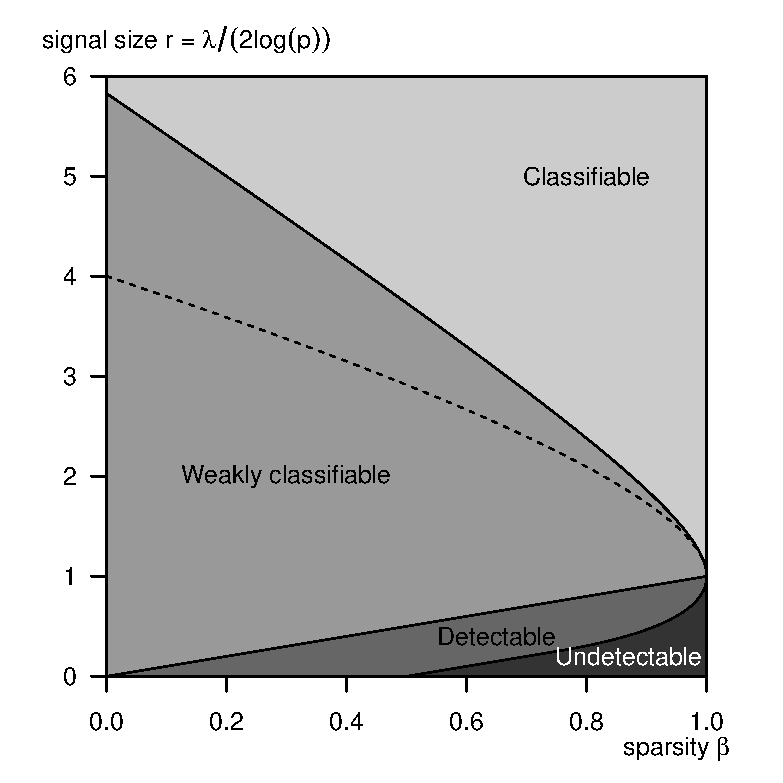
\includegraphics[width=0.7\textwidth]{./phase_diagram_chisquared.eps}
      % 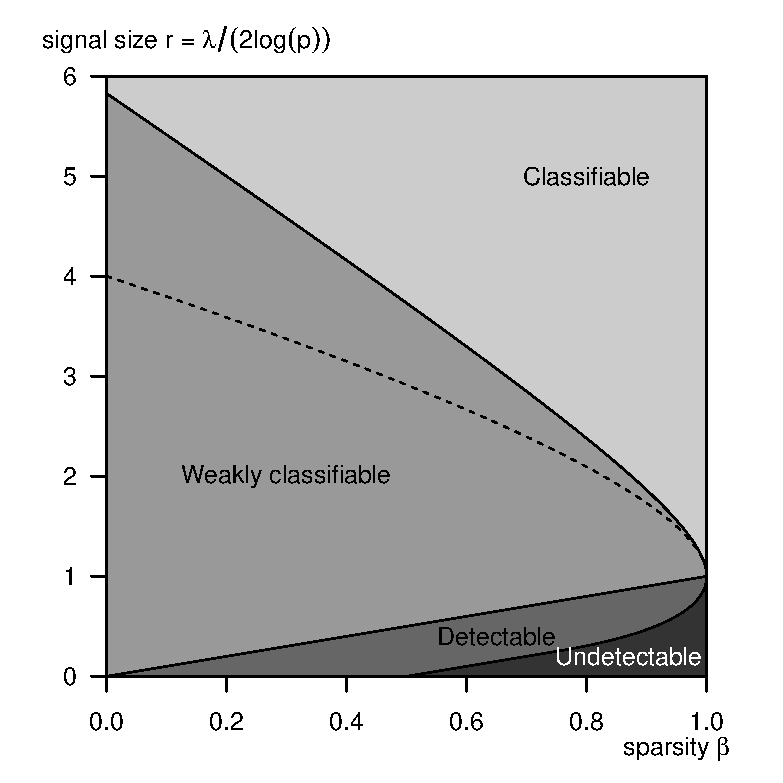
\includegraphics[width=0.35\textwidth]{./phase_diagram_chisquared.eps}
      \caption{The phase diagram of the high-dimensional chi-square model \eqref{eq:model-chisq}, illustrating the boundaries of the exact and approximate support recovery problems (Theorems \ref{thm:chi-squred-strong-boundary} and \ref{thm:chi-squred-weak-boundary}), and the signal detection problem (described in \citep{donoho2004higher}). 
      The risk of exact support recovery \eqref{eq:risk-exact} can be made to vanish above the strong classification boundary \eqref{eq:strong-classification-boundary-chisquared} in the \emph{classifiable} region; conversely, the risk has liminf at least one.
      Similarly, the risk of approximate support recovery \eqref{eq:risk-approximate} can be made to vanish above the weak classification boundary \eqref{eq:weak-classification-boundary-chisquared} in the \emph{weakly classifiable} region; conversely, the risk has liminf at least one.
      Both boundaries are unaffected by the degrees-of-freedom parameter in the model.
      } 
      \label{fig:phase-chi-squared}
\end{figure}

\begin{remark}
Remarkably, the degree-of-freedom parameter $\nu$ does not affect the boundary \eqref{eq:strong-classification-boundary-chisquared}.
In simulations, we find the approximation by the asymptotic boundary to be quite accurate even in moderate dimensions, and largely unaffected by the degrees of freedom.
See Section \ref{sec:numerical} for numerical illustrations.
\end{remark}

As alluded to in Section \ref{subsec:motivation-additive} in the introduction, Theorem \ref{thm:chi-squred-strong-boundary} also allows us to compare the difficulties of one-sided versus two-sided additives for additive models under Gaussian errors.

\begin{remark}
The exact support recovery problem under one-sided alternatives in the Gaussian additive error model \eqref{eq:model-additive} was studied \cite{gao2018fundamental}.
The same parametrization of sparsity \eqref{eq:signal-sparsity} was used.
The signal sizes of the non-zero mean shifts in $\mu(i)$ were parametrized in a similar fashion as \eqref{eq:signal-size} between $\sqrt{2\underline{r}\log{p}}$ and $\sqrt{2\overline{r}\log{p}}$, where $0<\underline{r}\le\overline{r}$.
Interestingly, under one-sided alternatives in the additive model, a phase transition in the $r$-$\beta$ plane also exists for the exact support recovery problem.
However, the boundary the phase transition is
\begin{equation} \label{eq:strong-classification-boundary-additive}
    \widetilde{g}(\beta) = \left(1 + \sqrt{1-\beta}\right)^2,
\end{equation}
which is strictly below that of two-sided case in \eqref{eq:strong-classification-boundary-chisquared}, except in the extremely sparse case $\beta = 1$.
In particular, as the problem becomes denser ($\beta\to0$), the required signal size in the one-sided additive model \eqref{eq:strong-classification-boundary-additive} approaches 2 since $\widetilde{g}(\beta)\to2$, while the required signal size in the chi-square (two-sided altenative additive) model \eqref{eq:strong-classification-boundary-chisquared} is almost two times higher, since ${g}(\beta)\to2\to3+2\sqrt{2}\approx 5.828$.
\end{remark}

\subsection{FDR-controlling procedures}
\label{subsec:FDR-controlling-procedures}

Recall the order statistics of our observations $x_{[1]} \ge x_{[2]}  \ge \ldots \ge x_{[p]}$.

\begin{definition}[Benjamini-Hochberg's procedure]
Let $i^*$ be the largest index such that
$$
\overline{F}(x_{[i]}) \le \alpha i/p.
$$
The Benjamini-Hochberg procedure with level $\alpha$ is the thresholding procedure with threshold
\begin{equation} \label{eq:BH-procedure}
    t_p(x) = x_{[i^*]},
\end{equation}
\end{definition}

This procedure is shown to control the FDR at level $\alpha$ when the statistics are
independent \cite{benjamini1995controlling}.

\subsection{The weak classification boundary}
\label{subsec:weak-classification-boundary}

Our second main result characterizes the phase-transition phenomenon in the approximate support recovery problem under the chi-square model.

\begin{theorem} \label{thm:chi-squred-weak-boundary}
Consider the high-dimensional chi-squared model \eqref{eq:model-chisq} with signal sparsity and size as described in \eqref{eq:signal-sparsity} and \eqref{eq:signal-size}.
The function 
\begin{equation} \label{eq:weak-classification-boundary-chisquared}
    h(\beta) = \beta
\end{equation}
characterizes the phase transition of approximate support recovery problem.
Specifically, if $\underline{r} > {h}(\beta)$, then the Benjamini-Hochberg procedure $\widehat{S}_p$ (defined in \eqref{eq:BH-procedure}) with FDR levels $\alpha=\alpha_p$ satisfying
\begin{equation} \label{eq:FDR-rate-to-zero}
    \alpha\to 0,\quad \text{and} \quad \alpha p^\delta\to\infty \text{  for any } \delta>0.
\end{equation}
achieves asymptotically approximate support recovery in the sense of \eqref{eq:approx-recovery-success}. 

Conversely, if $\overline{r} < {h}(\beta)$, then approximate support recovery asymptotically fails in the sense of \eqref{eq:approx-recovery-failure} for all thresholding procedures.
\end{theorem}

\begin{remark}
The approximate support recovery problem in the additive error model \eqref{eq:model-additive} was studied in \cite{arias2017distribution}, where a phase transition boundary was described in the sense of Definition \ref{def:approx-recovery-success-failure}.
Interestingly, the weak classification boundary under one-sided alternatives is the same as \eqref{eq:weak-classification-boundary-chisquared}.
Therefore, unlike exact support recovery, the requirement on the signal sizes in the approximate support recovery for the two-sided problem is no higher than in the one-sided case.

To complete the comparisons, we note that the phase transition boundary for sparse signal detection problem is also identical in both types of alternatives; this was analyzed in \cite{donoho2004higher}.
\end{remark}

\section{Odds ratio, rare variants, and signal sizes in association tests}
\label{sec:signal-size-odds-ratio}

In large scale variable screening studies, we would like to find suitable designs such that combinations of the dimensionality $p$, sparsity $\beta$, and signal sizes $r$ of the problem land in the desirable region of discovery, as predicted by the results in Section \ref{sec:chisq-boundaries}.

In practice, however, not all three of the parameters $(p, \beta, r)$ can be manipulated.
In particular, the problem dimensions and sparsity levels are usually determined by the underlying physical process.
In the GWAS example, the number of genomic marker locations is determined by the design of the chip used for sequencing, while the number of relevant genomic locations is a consequence of the biological process.
Therefore, in order to achieve a desired level of error control, one can only hope to influence the statistical signal sizes.

We discuss in this section how to attain the necessary statistical signal sizes in the case of association tests on 2-by-2 contingency tables, and clarify the relationship between statistical signal sizes and odds ratios in these tests.

\subsection{Odds ratios and statistical power}
\label{subsec:odds-and-power}

Although the non-centrality parameter $\lambda$ serves as a natural parameter for signal sizes in chi-square (and other omnidirectional) tests, its meaning is perhaps not as transparent.
A question frequently asked by practitioners is how signal sizes relate to odds ratios, commonly referred to as effect sizes in association tests.

Consider a 2-by-2 multinomial distribution with marginals probabilities $(\phi_1, \phi_2)$ and $(\theta_1, \theta_2)$, where $\phi_1 + \phi_2 = 1$ and $\theta_1 + \theta_2 = 1$.
\begin{center}
    \begin{tabular}{cccc}
    \hline
    & \multicolumn{2}{c}{Genotype} \\
    \cline{2-3}
    Probabilities & Variant 1 & Variant 2 & Total by phenotype \\
    \hline
    Cases & $\mu_{11}$ & $\mu_{12}$ & $\phi_1$ \\
    Controls & $\mu_{21}$ & $\mu_{22}$ & $\phi_2$ \\
    Total by genotype & $\theta_1$ & $\theta_2$ & 1 \\
    \hline
    \end{tabular}
\end{center}
The odds ratio is defined as the ratio of the phenotype frequencies between the two genotype variants,
\begin{equation} \label{eq:odds-ratio}
    \text{R} := \frac{\mu_{11}}{\mu_{21}}\Big/\frac{\mu_{12}}{\mu_{22}}
    = \frac{\mu_{11}\mu_{22}}{\mu_{12}\mu_{21}}.
\end{equation}
The multinomial distribution is fully parametrized by the trio $(\theta_1, \phi_1, R)$.
Independence between the genotypes and phenotyes would imply an odds ratio of zero, and hence
$$
\mu_{jk} = \phi_j\theta_k, \quad \text{for all }j,k \in\{1,2\}.
$$
When data are sampled from the multinomial distribution, the chi-square test defined in \eqref{eq:chisq-statistic} is asymptotically equivalent to tests including, e.g., the likelihood ratio test and Welch's t-test, both in terms of level and power \cite{ferguson2017course,gao2019upass}.

Specifically, with a sequence of local alternatives $\mu^{(1)}, \mu^{(2)}, \ldots$, such that $\sqrt{n}(\mu^{(n)}_{jk} - \phi_j\theta_k)$ converges to a constant table $\delta = (\delta_{jk})$, the aforementioned test statistics converge in distribution to the non-central chi-squared distribution with non-centrality parameter 
$$\lambda = \sum_{j=1}^2 \sum_{k=1}^2 {\delta_{jk}^2}/{(\phi_j\theta_k)}.$$
Therefore, for large samples from a fixed distribution $\mu$, the statistics would be well approximated by a $\chi^2_\nu(\lambda)$ distribution, where $\nu=1$ and
\begin{equation} 
    \lambda := n\sum_{j=1}^2 \sum_{k=1}^2 \frac{(\mu_{jk} - \phi_j\theta_k)^2}{\phi_j\theta_k}.
\end{equation}
Since $\lambda$ is linear in the number of samples $n$, we define 
\begin{equation} \label{eq:signal-size-chisq}
    w^2:=\lambda/n
\end{equation} 
as the signal size per sample.
Power of association tests at $\alpha$ level is approximately $\P[\chi^2_{\nu}(\lambda)>\chi^2_{\nu,\alpha}]$, where $\chi^2_{\nu,\alpha}$ is the upper $\alpha$-quantile of a central Chi-squared distribution.
Power calculations would therefore only depend on the distributions through $\lambda=nw^2$, and statistical power is increasing in the signal sizes per sample $w^2$.
The relationship between the $w^2$ and the odds ratio $\text{R}$ is characterized in the following proposition.

\begin{proposition} \label{prop:signal-size-odds-ratio}
Consider 2-by-2 multinomial distribution with marginals $(\phi_1, \phi_2)$ and $(\theta_1, \theta_2)$.
Let signal size $w^2$ be defined as in \eqref{eq:signal-size-chisq}, and odds ratio $\text{R}$ be defined as in \eqref{eq:odds-ratio}. 
Then we have $w^2 = 0$ if $R=1$, and
\begin{equation} \label{eq:signal-size-odds-ratio}
    w^2(\text{R}) =
    \frac{1}{4A(\text{R}-1)^2}\left(B+CR-\sqrt{(B+CR)^2-4A(R-1)^2}\right)^2,
\end{equation}
if $R\neq1$, and $R>0$, 
with constants $A = \phi_1\theta_1\phi_2\theta_2$, $B = \phi_1\theta_1+\phi_2\theta_2$, and $C = \phi_1\theta_2+\phi_2\theta_1$.
\end{proposition}

We illustrate Relation \eqref{eq:signal-size-odds-ratio} for selected values of marginals $\theta_1$ and $\phi_1$ in Figure \ref{fig:signal-vs-odds}.
Notice that while the odds ratio $R$ can be unbounded for any arbitrary marginal distributions, the signal sizes $w^2$ are bounded from above by constants that depend only on the marginals $\phi_1$ and $\theta_1$.
This is quantified in the next corollary.

\begin{figure}
      \centering
      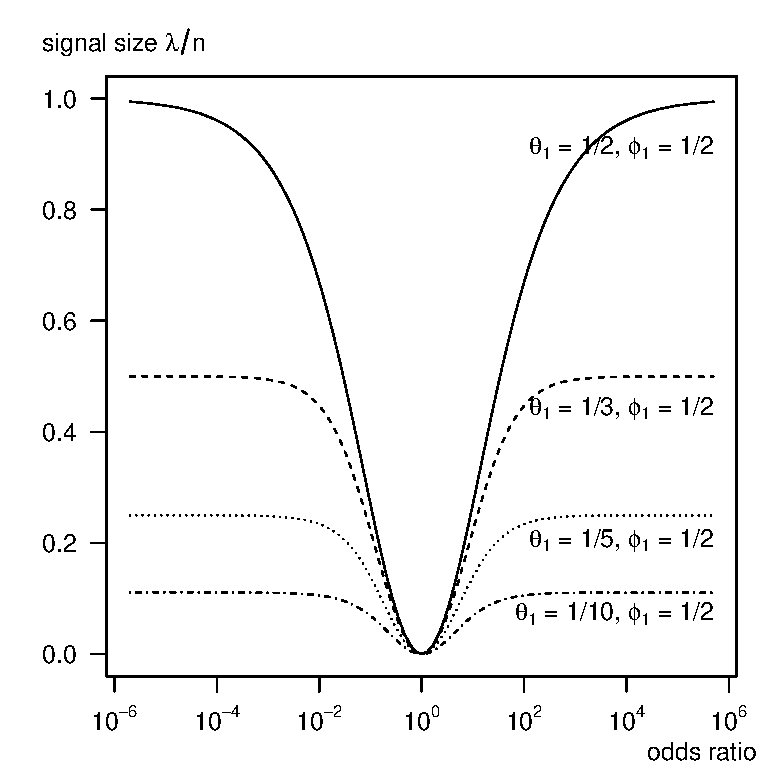
\includegraphics[width=0.49\textwidth]{./singal-vs-odds-p05}
      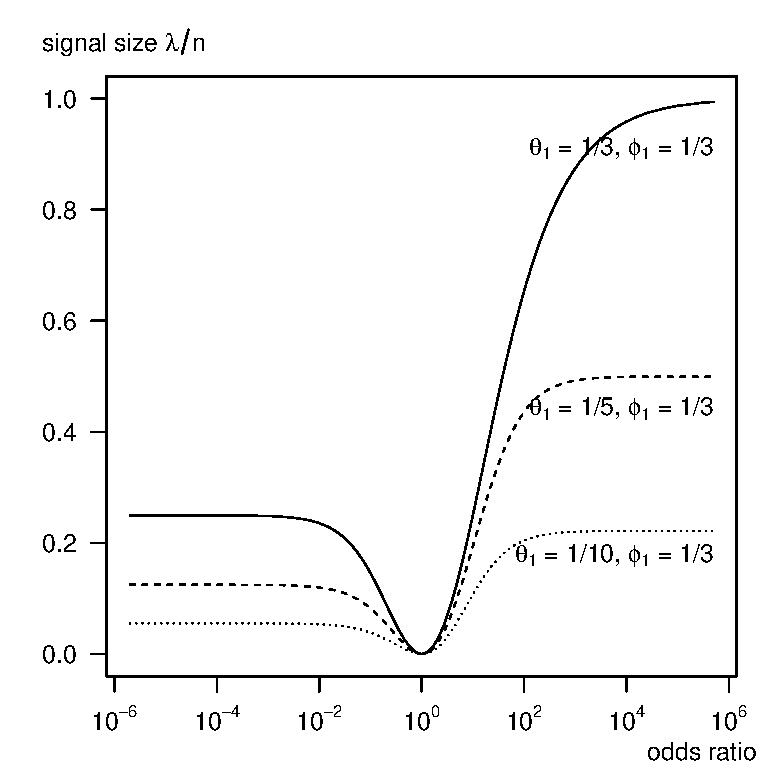
\includegraphics[width=0.49\textwidth]{./singal-vs-odds-p0333}            
      % 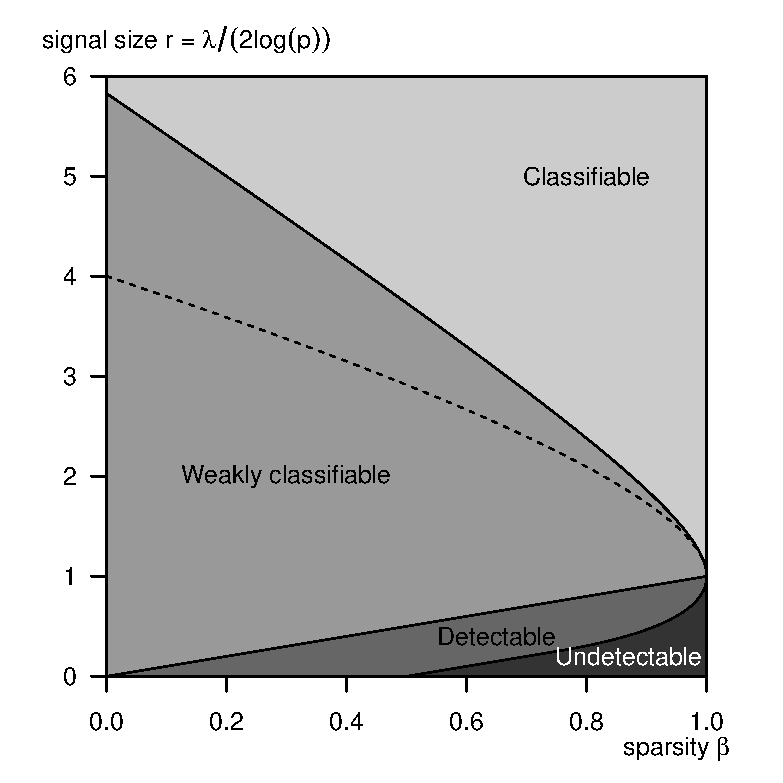
\includegraphics[width=0.35\textwidth]{./phase_diagram_chisquared.eps}
      \caption{Signal size in chi-square tests as functions of odds ratio in 2-by-2 multinomial distributions, for selected marginal probabilities; see Relation \eqref{eq:signal-size-odds-ratio} in Proposition \ref{prop:signal-size-odds-ratio}.
      For fixed marginal distributions, extreme odds ratios imply stronger signals at a given sample size.
      However, the signal sizes are bounded above by constants that depend on the marginal distributions; see Relation \eqref{eq:signal-size-upper-bound}.
      % Unbalanced marginal distributions -- or rare variants -- lead to smaller signal sizes at a given odds ratio.
      } 
      \label{fig:signal-vs-odds}
\end{figure}

\begin{corollary} \label{cor:signal-limits-OR}
The signal size as a function of the odds ratio $w^2(R)$ is decreasing on $(0,1)$ and increasing on $(1,\infty)$, with limits
\begin{equation} \label{eq:signal-size-upper-bound-1}
    \lim_{\text{R}\to0_+} w^2(\text{R}) = \min\left\{\frac{\phi_1\theta_1}{\phi_2\theta_2}, \frac{\phi_2\theta_2}{\phi_1\theta_1}\right\},
\end{equation}
and
\begin{equation} \label{eq:signal-size-upper-bound-2}
    \lim_{\text{R}\to+\infty} w^2(\text{R}) = \min\left\{\frac{\phi_1\theta_2}{\phi_2\theta_1}, \frac{\phi_2\theta_1}{\phi_1\theta_2}\right\}.
\end{equation}
\end{corollary}


\subsection{Rare variants and the optimal study design}
\label{subsec:optimal-design} 


We make the important distinction here between the marginal distributions of genotypes and phenotypes \emph{in subjects of the study}, versus the marginal distributions \emph{in the general population}.
Throughout this paper marginal distributions refer to the quantities \emph{in the study}.
As we will see in Section \ref{subsec:odds-and-power}, only the quantities in the study are relevant for statistical power, while quantities in the population do not play a role.

Typically in a genetic study, the marginal distribution of the phenotypes can be pre-determined.
That is, we are able to decide on the number of recruited subjects in cases and controls.
In contrast, the marginal distribution of the genotypes in the study are typically unknown a priori. 
On the other hand, the conditional distributions of the genetic variants in the healthy control groups are sometimes known.
We will see in Section \ref{subsec:optimal-design} that this information on the conditional distributions will allow us to determine the optimal proportion of cases versus controls in a study.


While the marginal distributions of alleles $(\theta_1, \theta_2)$ are often unknown before collecting the data, their conditional distributions in the healthy control group can sometimes be estimated from prior studies.
We denote the conditional frequency of the first allele among the subjects in the control group as
$$
f := \mu_{21} / \phi_2.
$$
Since we can always relabel the variants, we may assume without loss of generality that the first variant is associated with an increased risk of disease, and is henceforth referred to as the risk allele.
We shall also refer to a risk allele with very low frequency in the control group (i.e., $f\approx 0$) as a rare variant.

Just as the multinomial distribution is fully parametrized by the marginals and odds ratio  $(\theta_1, \phi_1, R)$, it can also be fully described by the conditional frequency of allele in the control group $f$, proportion of cases in the study $\phi_1$, and the odds ratio $R$.

\begin{center}
    \begin{tabular}{cccc}
    \hline
    & \multicolumn{2}{c}{Genotype} \\
    \cline{2-3}
    Probabilities & Variant 1 & Variant 2 & Total by phenotype \\
    \hline
    Cases & $\frac{\phi_1fR}{(fR+1-f)}$ & $\frac{\phi_1(1-f)}{(fR+1-f)}$ & $\phi_1$ \\
    Controls & $f(1-\phi_1)$ & $(1-f)(1-\phi_1)$ & $1-\phi_1$ \\
    \hline
    \end{tabular}
\end{center}

Proposition \ref{prop:signal-size-odds-ratio} may then be re-stated in terms of the new trio $(f, \phi_1, R)$.

% Note that all these quantities refer to what is in the study, and differ from their counterparts in the general population.

\begin{corollary} \label{cor:signal-size-odds-ratio-conditional-frequency}
In the 2-by-2 multinomial distribution with marginals $(\phi_1, \phi_2 = 1-\phi_1)$, and conditional distribution of the variants in the control group $(f, 1-f)$,
Relation \eqref{eq:signal-size-odds-ratio} holds with $\theta_1 = {\phi_1fR}/{(fR+1-f)} + f(1-\phi_1)$ and $\theta_2 = 1-\theta_1$.
\end{corollary} 



\section{Numerical illustrations}
\label{sec:numerical}

We illustrate the phase-transition phenomena in finite dimensions with numerical experiments.
% We also demonstrate the fundamental trade-off between odds ratios and relative frequencies in association studies, as outlined in Proposition \ref{prop:signal-size-odds-ratio} and Corollary \ref{cor:signal-size-odds-ratio-conditional-frequency}, using evidence from large-scale genetic studies.

\subsection{The exact support recovery problem}

The sparsity and signal size of the sparse mean vector in the experiments are parametrized as in \eqref{eq:signal-sparsity} and \eqref{eq:signal-size}, with signal sizes assumed equal.
We estimate the support set $S$ with using Bonferroni's procedure, where the nominal FWER level for Bonferroni's procedures are set at $1/(5{\log{p}})$, in line with the assumptions in Theorem \ref{thm:chi-squared-exact-boundary}.
Experiments were repeated 1000 times at each of the 400 sparsity-and-signal-size combinations, for dimensions $p=10^2, 10^3$, and $10^4$.

The empirical probabilities of exact support recovery under Bonferroni's procedure are shown in Figure \ref{fig:phase-simulated-chi-squared}.
The numerical results suggest not only good accuracy of the predicted boundaries in high-dimensions ($p=10^4$, right panels of Figure \ref{fig:phase-simulated-chi-squared}), but also practical relevance even at moderate dimensions ($p=100$, left panels of Figure \ref{fig:phase-simulated-chi-squared}).

\begin{figure}
      \centering
      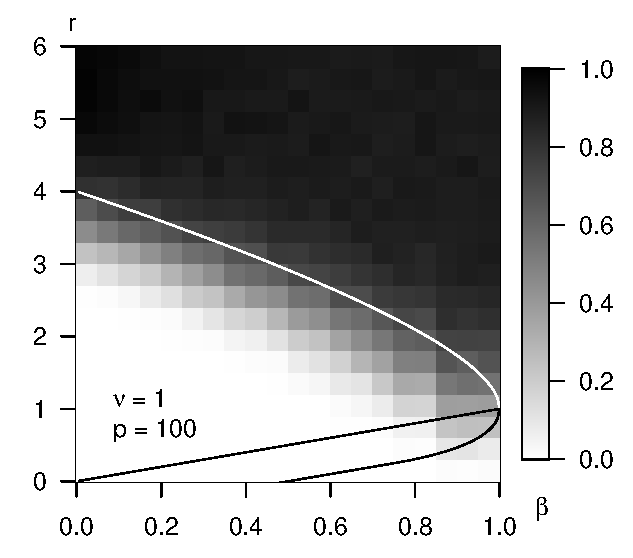
\includegraphics[width=0.32\textwidth]{./sim_strong_boundary/simulated_phase_diagram_chi-squared_nu1_p100.eps}
      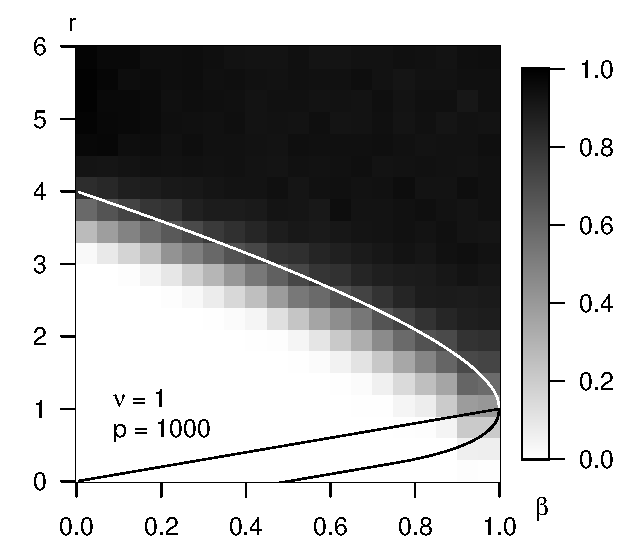
\includegraphics[width=0.32\textwidth]{./sim_strong_boundary/simulated_phase_diagram_chi-squared_nu1_p1000.eps}
      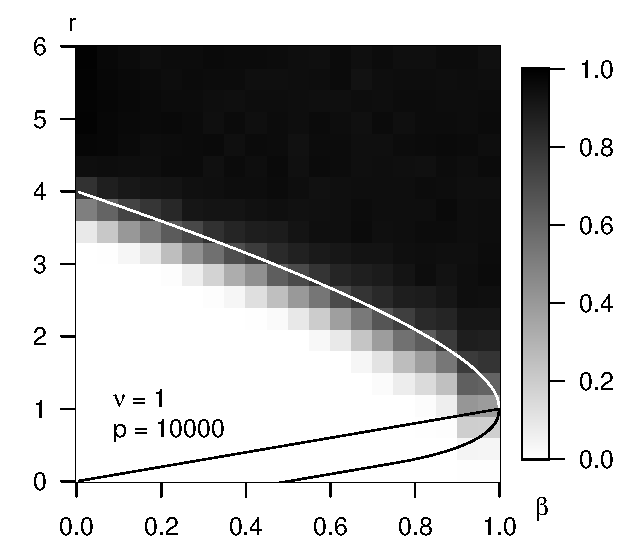
\includegraphics[width=0.32\textwidth]{./sim_strong_boundary/simulated_phase_diagram_chi-squared_nu1_p10000.eps}
      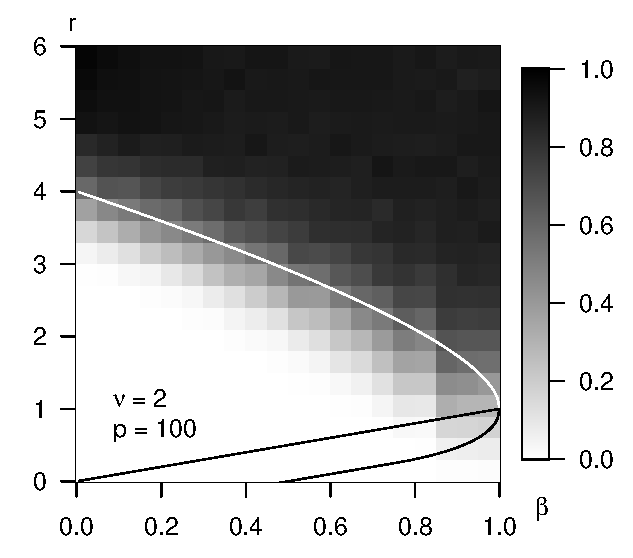
\includegraphics[width=0.32\textwidth]{./sim_strong_boundary/simulated_phase_diagram_chi-squared_nu2_p100.eps}
      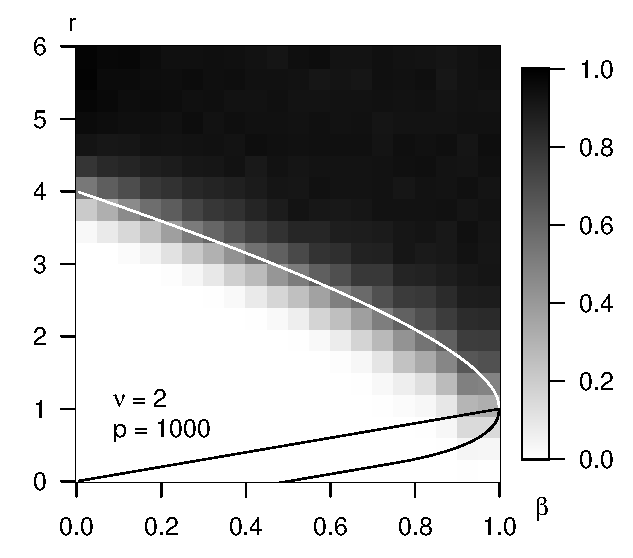
\includegraphics[width=0.32\textwidth]{./sim_strong_boundary/simulated_phase_diagram_chi-squared_nu2_p1000.eps}
      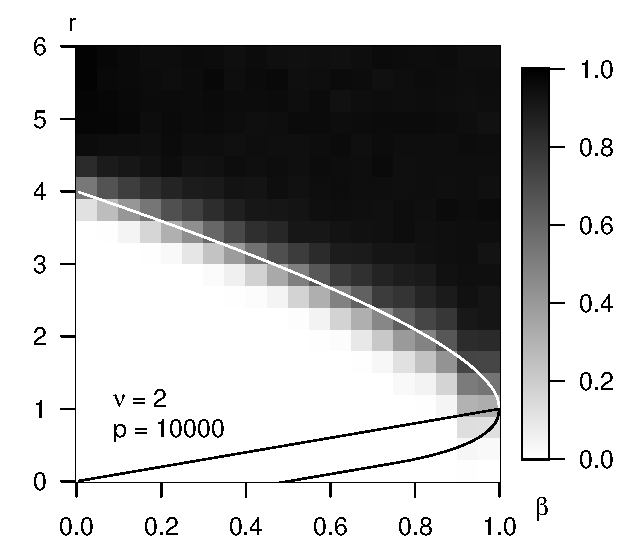
\includegraphics[width=0.32\textwidth]{./sim_strong_boundary/simulated_phase_diagram_chi-squared_nu2_p10000.eps}
      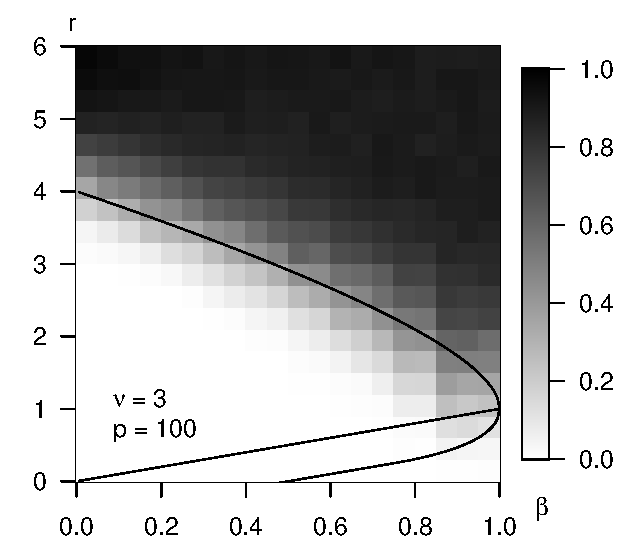
\includegraphics[width=0.32\textwidth]{./sim_strong_boundary/simulated_phase_diagram_chi-squared_nu3_p100.eps}
      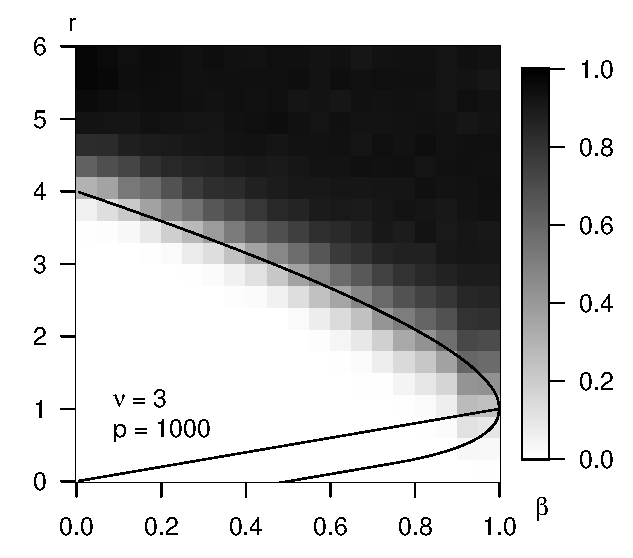
\includegraphics[width=0.32\textwidth]{./sim_strong_boundary/simulated_phase_diagram_chi-squared_nu3_p1000.eps}
      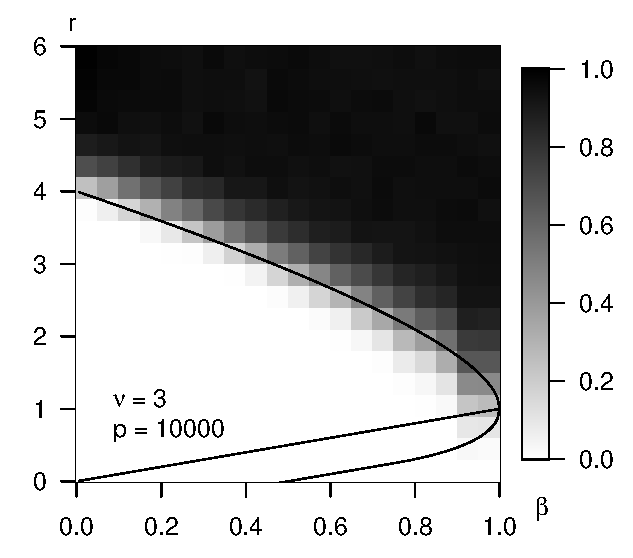
\includegraphics[width=0.32\textwidth]{./sim_strong_boundary/simulated_phase_diagram_chi-squared_nu3_p10000.eps}
      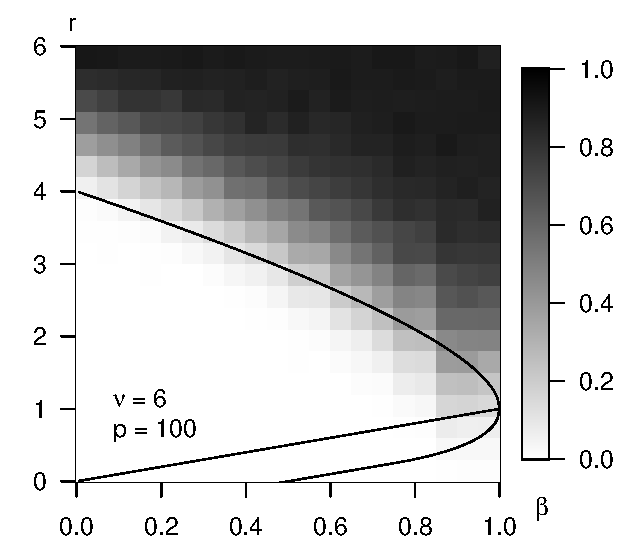
\includegraphics[width=0.32\textwidth]{./sim_strong_boundary/simulated_phase_diagram_chi-squared_nu6_p100.eps}
      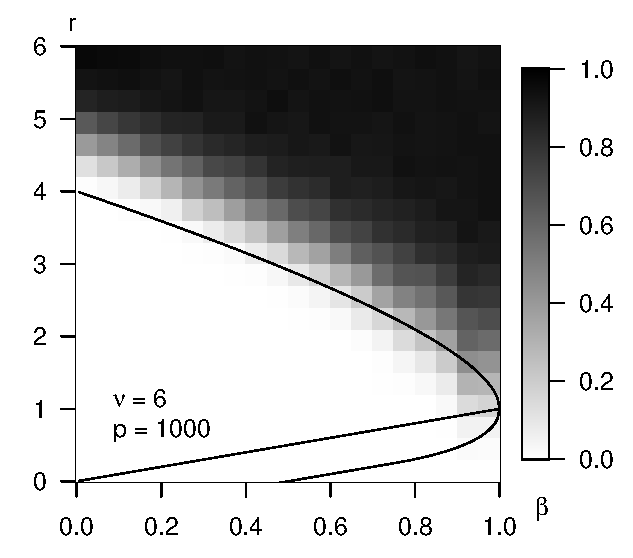
\includegraphics[width=0.32\textwidth]{./sim_strong_boundary/simulated_phase_diagram_chi-squared_nu6_p1000.eps}
      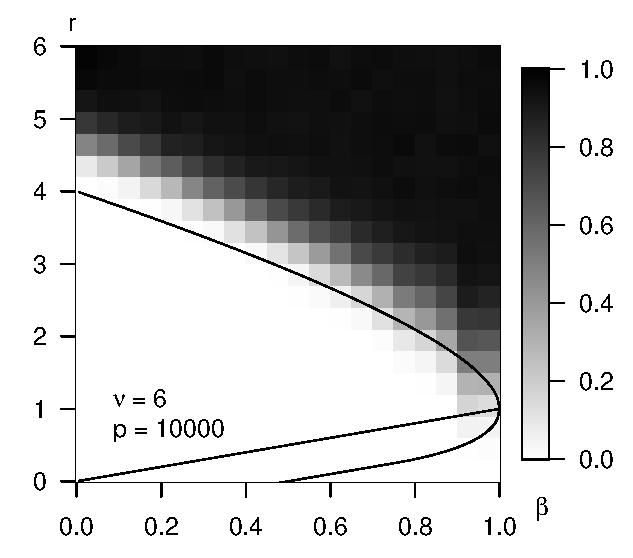
\includegraphics[width=0.32\textwidth]{./sim_strong_boundary/simulated_phase_diagram_chi-squared_nu6_p10000.eps}
      \caption{The empirical probability of exact support recovery using Bonferroni's procedure in the chi-squared model \eqref{eq:model-chisq}. 
      We simulate $\nu=1, 2, 3, 6$ (first to last row), at dimensions $p=10^2, 10^3, 10^4$ (left to right column), for a grid of sparsity levels $\beta$ and signal sizes $r$.
      The experiments were repeated 1000 times for each sparsity-signal size combination; darker color indicates higher probability of exact support recovery.  
      Numerical results are generally in agreement with the boundaries described in Theorem \ref{thm:chi-squared-exact-boundary}; for large $\nu$'s, the phase transitions take place somewhat above the predicted boundaries.
      The boundary for the approximate support recovery (Theorem \ref{thm:chi-squared-approx-boundary}) and the detection boundary (see \citep{donoho2004higher}) are plotted for comparison.} 
      \label{fig:phase-simulated-chi-squared}
\end{figure}

We conduct further experiments to examine the optimality claims in Theorem \ref{thm:chi-squared-exact-boundary} by comparing with the oracle procedure with thresholds $t_p=\min_{i\in S}x(i)$.
We also examine the claims in Remark \ref{rmk:strong-classification-boundary-1}, and compare the one-sided alternatives in Gaussian additive models with the two-sided alternatives (or equivalently, the chi-square model with $\nu=1$).
We apply both Bonferroni's procedure and the oracle thresholding procedure in both settings.

Experiments were repeated 1000 times for signal sizes ranging from $r=0$ to $6$, and for dimensions $10^2, 10^3$, and $10^5$.
Results of the experiments, shown in Figure \ref{fig:one-vs-two-sided-exact_support_recovery}, suggest vanishing difference between difficulties of two-sided vs one-sided alternatives in the additive error models, as well as vanishing difference between the powers of Bonferroni's procedures and the oracle procedures.

\begin{figure}
      \centering
      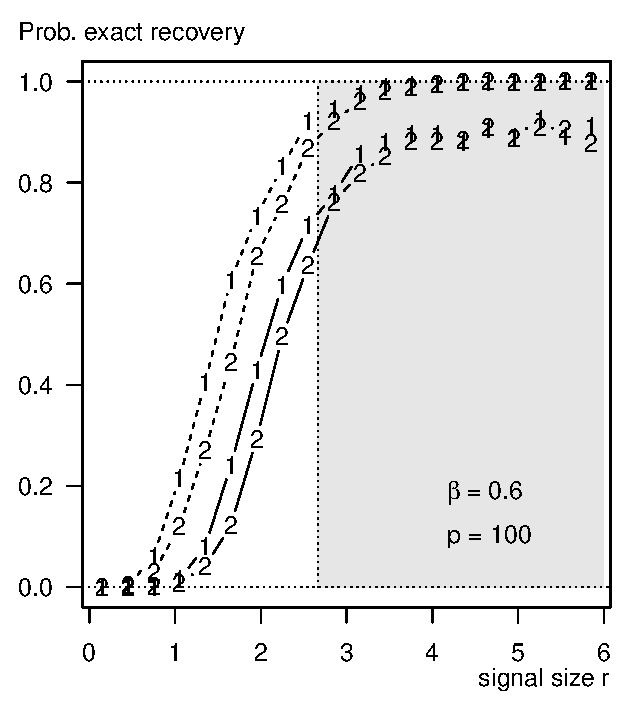
\includegraphics[width=0.32\textwidth]{./sim_one-vs-two-sided/exact_recovery_one-vs-two-sided_beta06_p100.eps}
      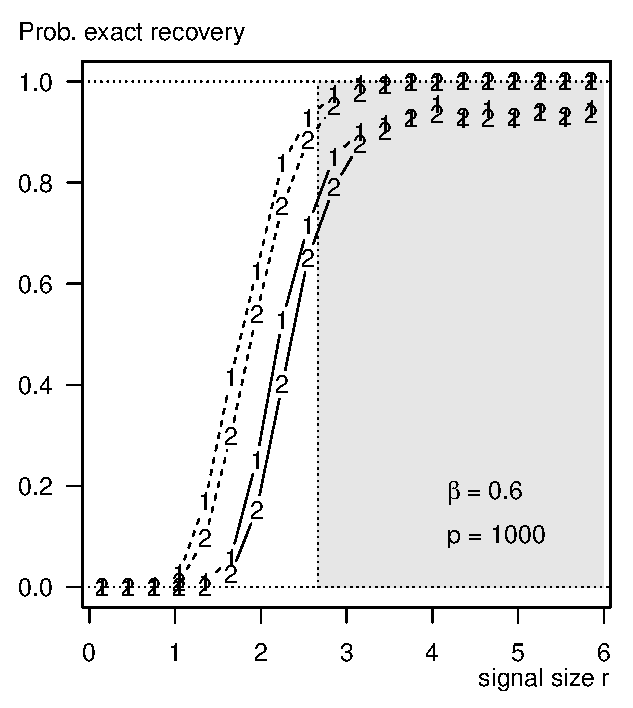
\includegraphics[width=0.32\textwidth]{./sim_one-vs-two-sided/exact_recovery_one-vs-two-sided_beta06_p1000.eps}
      % 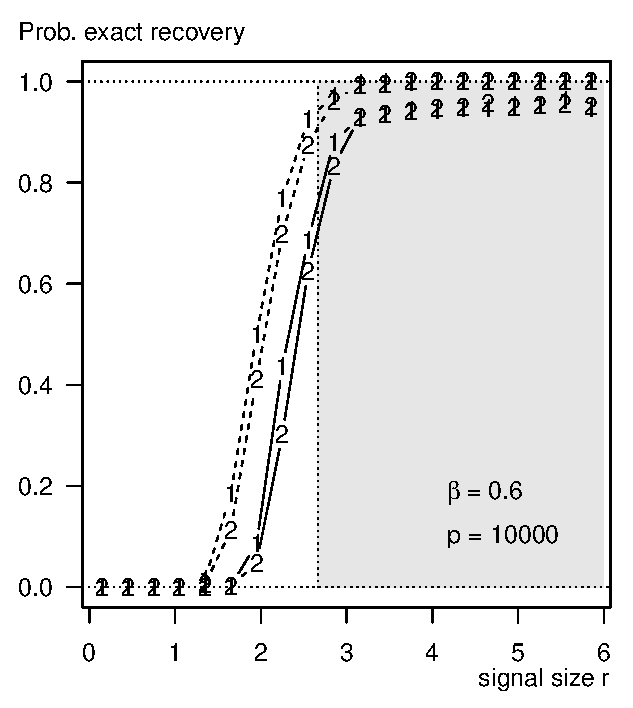
\includegraphics[width=0.33\textwidth]{./sim_one-vs-two-sided/exact_recovery_one-vs-two-sided_beta06_p10000.eps}
      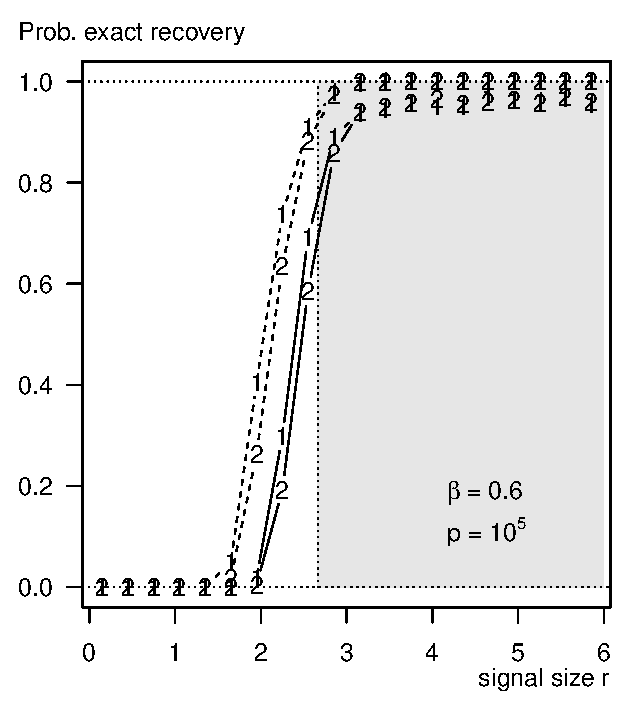
\includegraphics[width=0.32\textwidth]{./sim_one-vs-two-sided/exact_recovery_one-vs-two-sided_beta06_p100000.eps}
      \caption{The empirical probability of exact support recovery using Bonferroni's procedure (solid curves) and the oracle procedure (dashed curves) in the chi-squared model with $\nu=1$ (marked `2') and under one-sided alternatives in the additive Gaussian error model (marked `1'). 
      We simulate at dimensions $p=10^2, 10^3, 10^5$ (left to right) for a grid of signal sizes $r$ and sparsity level $\beta=0.6$.
      The experiments were repeated 1000 times for each method-model-signal-size combination. 
      Numerical results show evidence of convergence to the 0-1 law predicted by Theorem \ref{thm:chi-squared-exact-boundary}; regions where exact support recovery is asymptotically achievable are shaded in grey.
      The difference in power between Bonferroni's procedure and the oracle procedure, as well as in the two types of alternatives both decrease as dimensionality increases.} 
      \label{fig:one-vs-two-sided-exact_support_recovery}
\end{figure}

\subsection{The approximate, and approximate-exact support recovery problem}

Similar experiments are conducted to examine the optimality claims in Theorem \ref{thm:chi-squared-approx-boundary}, and in Remark \ref{rmk:weak-classification-boundary}.
The oracle procedure for approximate support recovery is defined to be the thresholding procedure with threshold
$$
t_p(x, S) \in \argmin_{t\in\R} \frac{|\widehat{S}(t)\setminus S|}{\max\{|\widehat{S}(t)|,1\}} + \frac{|S\setminus \widehat{S}(t)|}{\max\{|{S}|,1\}},
%\mathcal{R^\mathrm{oracle}} \in \argmin_{\widehat{S}(\mathcal{R})\in\mathcal{S}} \mathrm{risk}^{\mathrm{A}}(\mathcal{R}),
$$
where $\widehat{S}(t) = \{i\;|\;x(i)\ge t\}$;
in implementation, we need only scan the values of observations $t\in\{x(1), \ldots, x(p)\}$. 
The nominal FDR level for the BH procedure is set at $1/(5{\log{p}})$, satisfying the assumptions in Theorem \ref{thm:chi-squared-approx-boundary}; all other parameters are identical to that in the experiments for exact support recovery.
Results of the experiments are shown in Figure \ref{fig:one-vs-two-sided-approx_support_recovery} and Figure \ref{fig:phase-simulated-chi-squared-approx-boundary}.

We also examine the boundary described in Theorem \ref{thm:chi-squared-exact-approx-boundary}.
All experimental settings are identical to that in the experiments for approximate support recovery.
Results of the experiments are shown in Figure \ref{fig:phase-simulated-chi-squared-approx-exact-boundary}.
% Results for the BH procedure are in general close to that of the oracle procedure, 
We also compare the performance of the BH procedure with an oracle procedure with threshold
$$
t_p(x, S) \in \min_{i\in S} x(i).
$$
In experiments, we noticed that the BH procedure sets its threshold somewhat higher than the oracle, especially for small $\beta$'s. 
The phase transition for the oracle procedure (excluded in the interest of space) follows much more closely the predicted boundary \eqref{eq:approx-exact-boundary-chisquared}.

\begin{figure}
      \centering
      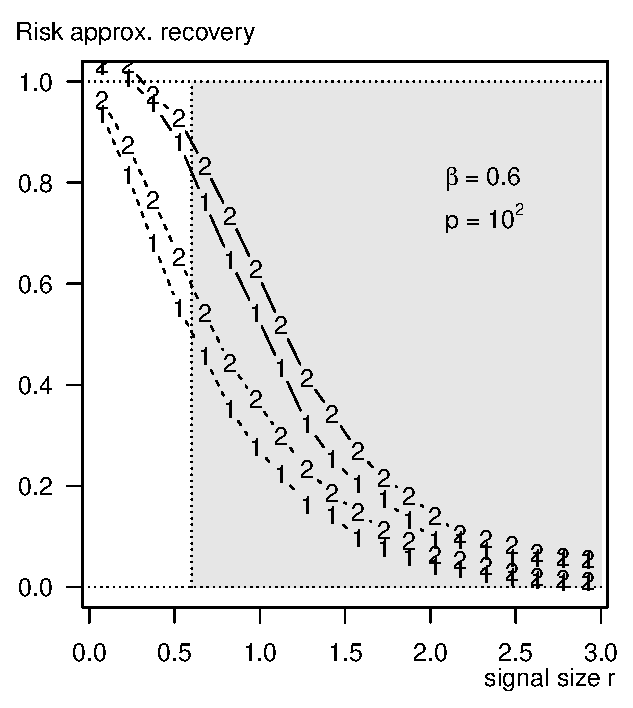
\includegraphics[width=0.32\textwidth]{./sim_one-vs-two-sided/approx_recovery_one-vs-two-sided_beta06_p100.eps}
      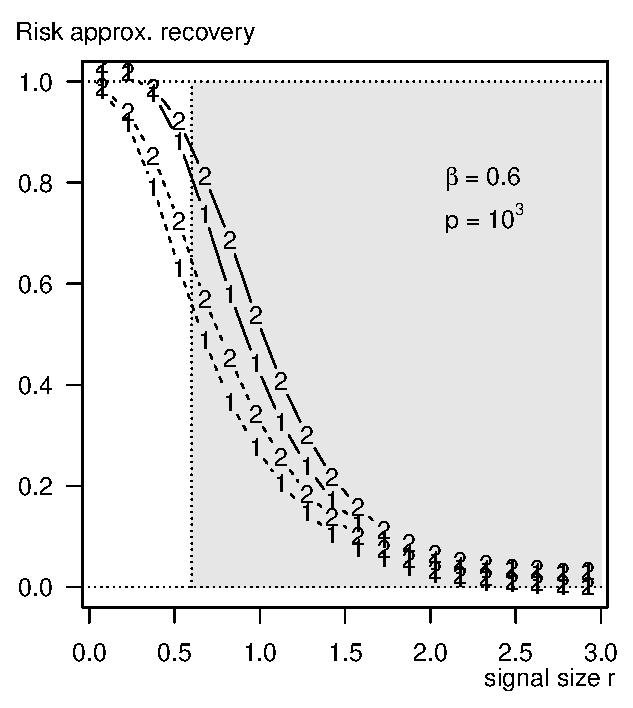
\includegraphics[width=0.32\textwidth]{./sim_one-vs-two-sided/approx_recovery_one-vs-two-sided_beta06_p1000.eps}
      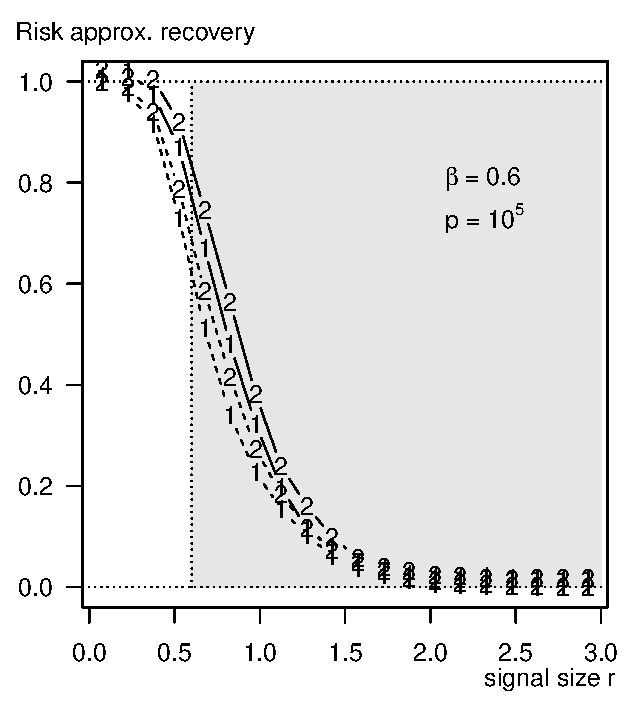
\includegraphics[width=0.32\textwidth]{./sim_one-vs-two-sided/approx_recovery_one-vs-two-sided_beta06_p100000.eps}
      \caption{The empirical risk of approximate support recovery using Benjamini-Hochberg's procedure (solid curves) and the oracle procedure (dashed curves) in the chi-squared model with $\nu=1$ (marked `2') and under one-sided alternatives in the additive Gaussian error model (marked `1'). 
      We simulate at dimensions $p=10^2, 10^3, 10^5$ (left to right) for a grid of signal sizes $r$ and sparsity level $\beta=0.6$.
      The experiments were repeated 1000 times for each method-model-signal-size combination. 
      Numerical results show evidence of convergence to the 0-1 law predicted by Theorem \ref{thm:chi-squared-approx-boundary}; regions where approximate support recovery is asymptotically achievable are shaded in grey.
      The difference in power between Benjamini-Hochberg's procedure and the oracle procedure, as well as in the two types of alternatives both decrease as dimensionality increases.} 
      \label{fig:one-vs-two-sided-approx_support_recovery}
\end{figure}


\begin{figure}
      \centering
      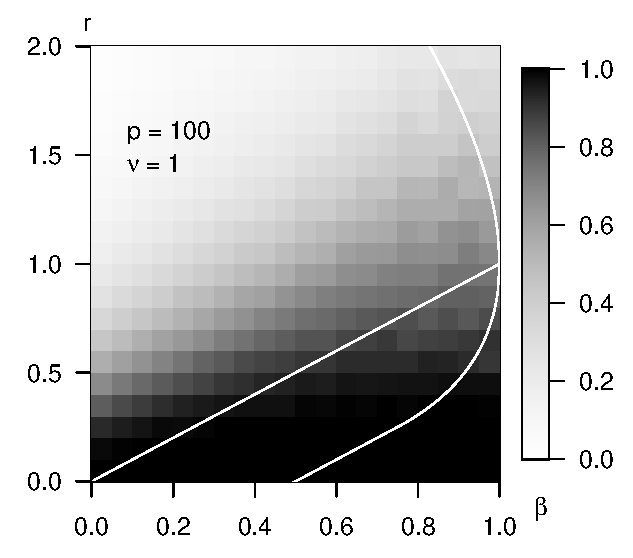
\includegraphics[width=0.32\textwidth]{./sim_weak_boundary/simulated_weak_boundary_chi-squared_nu1_p100.eps}
      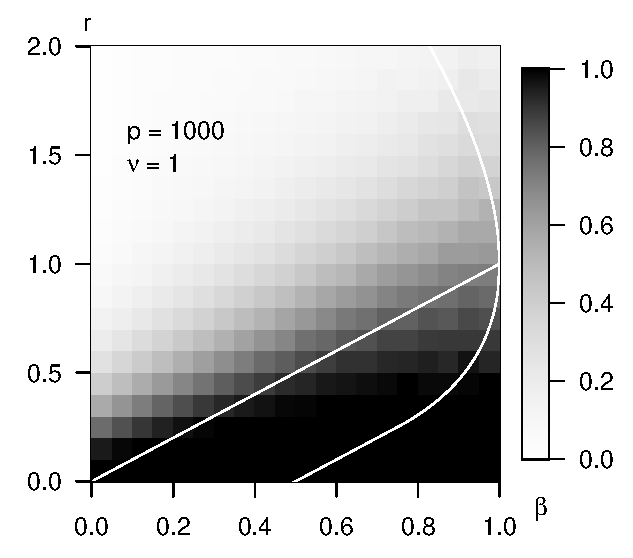
\includegraphics[width=0.32\textwidth]{./sim_weak_boundary/simulated_weak_boundary_chi-squared_nu1_p1000.eps}
      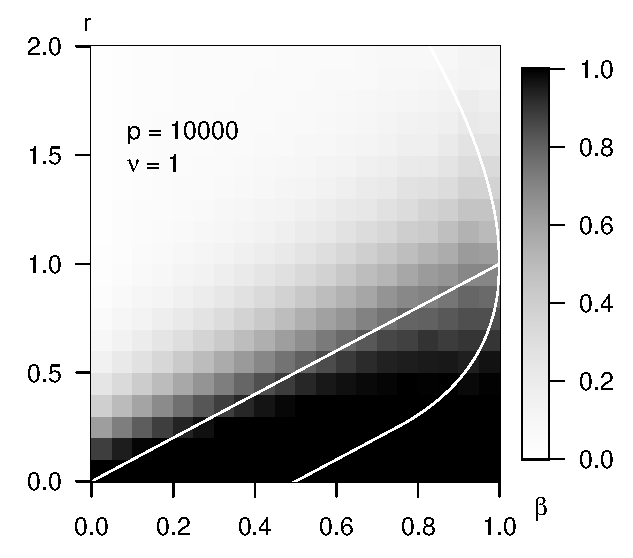
\includegraphics[width=0.32\textwidth]{./sim_weak_boundary/simulated_weak_boundary_chi-squared_nu1_p10000.eps}
      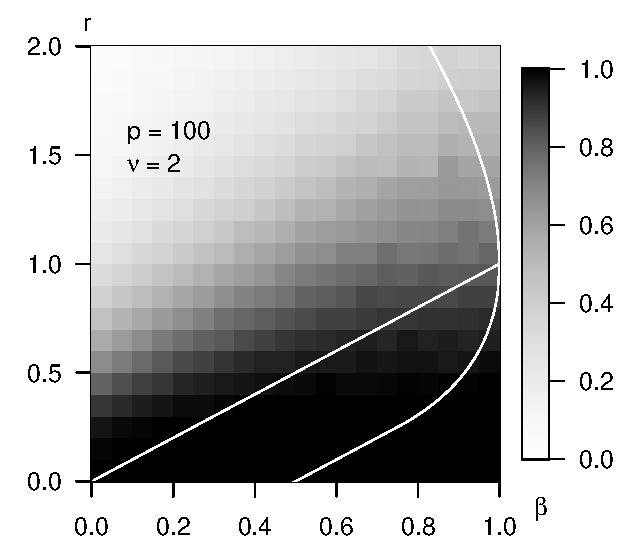
\includegraphics[width=0.32\textwidth]{./sim_weak_boundary/simulated_weak_boundary_chi-squared_nu2_p100.eps}
      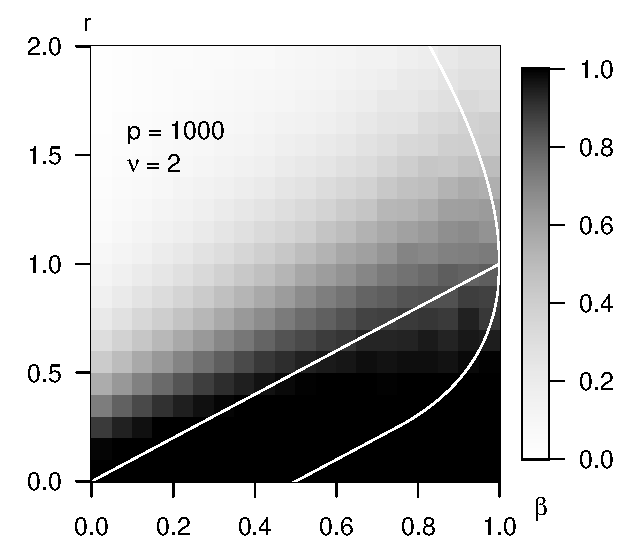
\includegraphics[width=0.32\textwidth]{./sim_weak_boundary/simulated_weak_boundary_chi-squared_nu2_p1000.eps}
      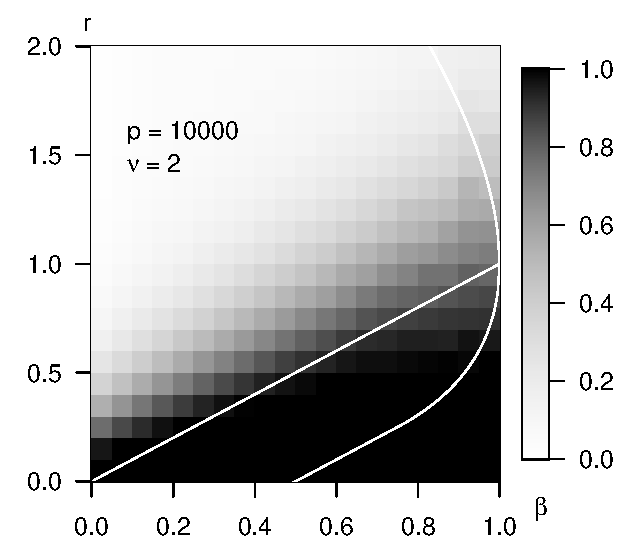
\includegraphics[width=0.32\textwidth]{./sim_weak_boundary/simulated_weak_boundary_chi-squared_nu2_p10000.eps}
      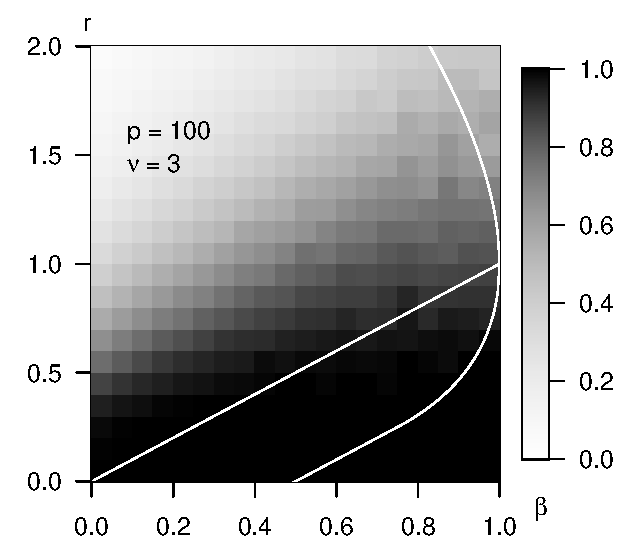
\includegraphics[width=0.32\textwidth]{./sim_weak_boundary/simulated_weak_boundary_chi-squared_nu3_p100.eps}
      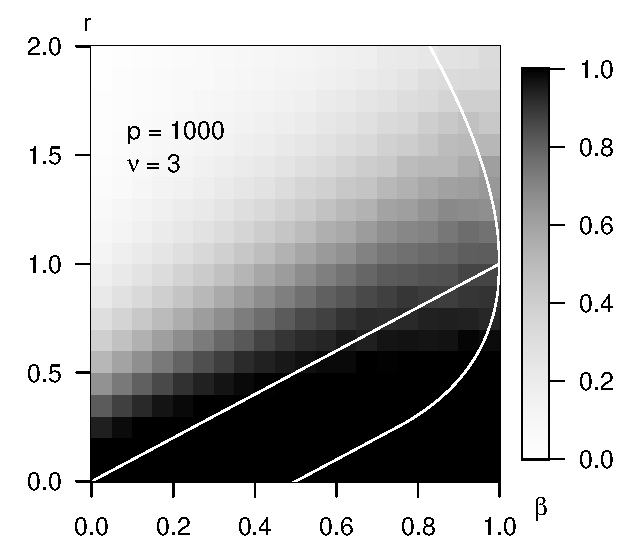
\includegraphics[width=0.32\textwidth]{./sim_weak_boundary/simulated_weak_boundary_chi-squared_nu3_p1000.eps}
      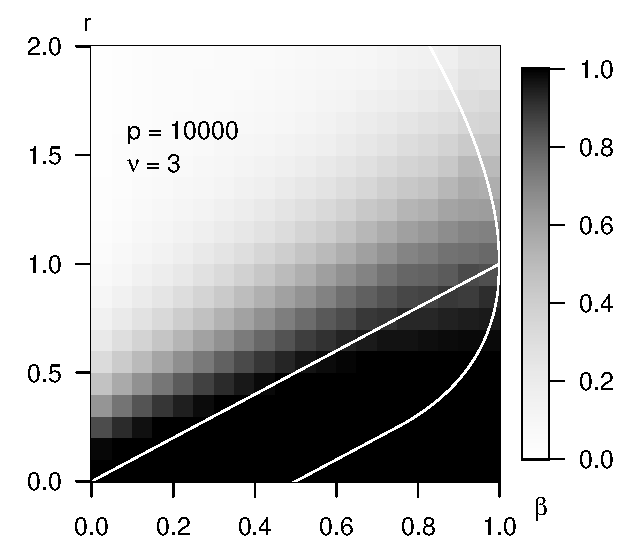
\includegraphics[width=0.32\textwidth]{./sim_weak_boundary/simulated_weak_boundary_chi-squared_nu3_p10000.eps}
      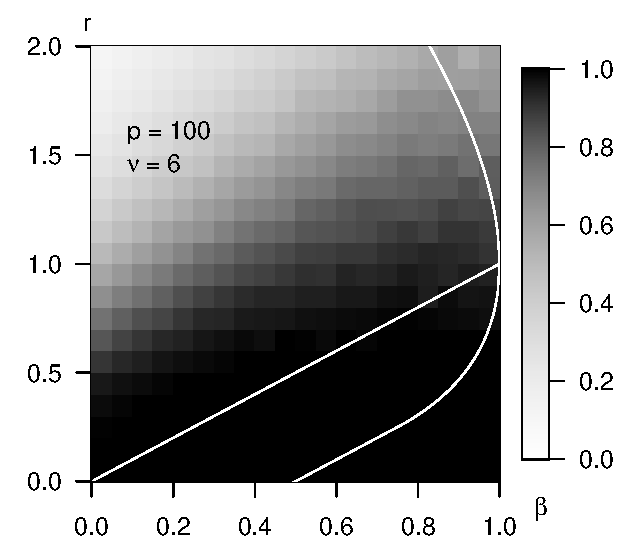
\includegraphics[width=0.32\textwidth]{./sim_weak_boundary/simulated_weak_boundary_chi-squared_nu6_p100.eps}
      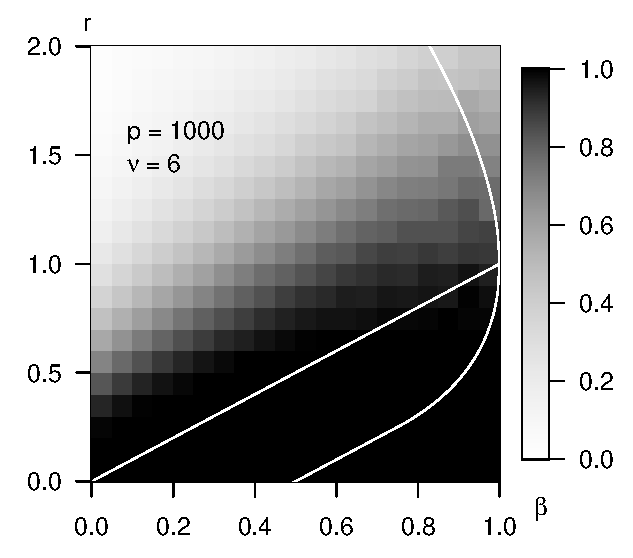
\includegraphics[width=0.32\textwidth]{./sim_weak_boundary/simulated_weak_boundary_chi-squared_nu6_p1000.eps}
      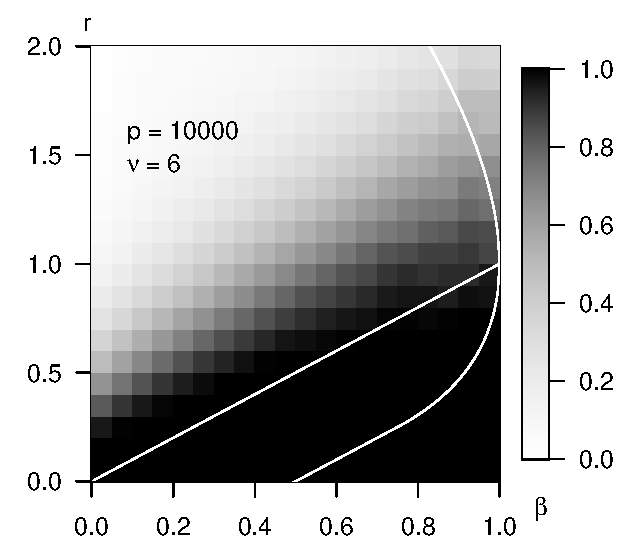
\includegraphics[width=0.32\textwidth]{./sim_weak_boundary/simulated_weak_boundary_chi-squared_nu6_p10000.eps}
      \caption{The estimated risk of approximate support recovery $\mathrm{risk}^{\mathrm{A}}$ (see \eqref{eq:risk-approximate}) of the Benjamini-Hochberg procedure in the chi-squared model \eqref{eq:model-chisq}. 
      We simulate $\nu=1, 2, 3, 6$ (first to last row), at dimensions $p=10^2, 10^3, 10^4$ (left to right column), for a grid of sparsity levels $\beta$ and signal sizes $r$.
      The experiments were repeated 1000 times for each sparsity-signal size combination; darker color indicates higher larger $\mathrm{risk}^{\mathrm{A}}$. 
      Numerical results are generally in agreement with the boundaries described in Theorem \ref{thm:chi-squared-approx-boundary}; for large $\nu$'s, the phase transitions take place somewhat above the predicted boundaries.
      The boundary for the exact support recovery problem (Theorem \ref{thm:chi-squared-exact-boundary}) and the detection boundary (see \citep{donoho2004higher}) are plotted for comparison.} 
      \label{fig:phase-simulated-chi-squared-approx-boundary}
\end{figure}


\begin{figure}
      \centering
      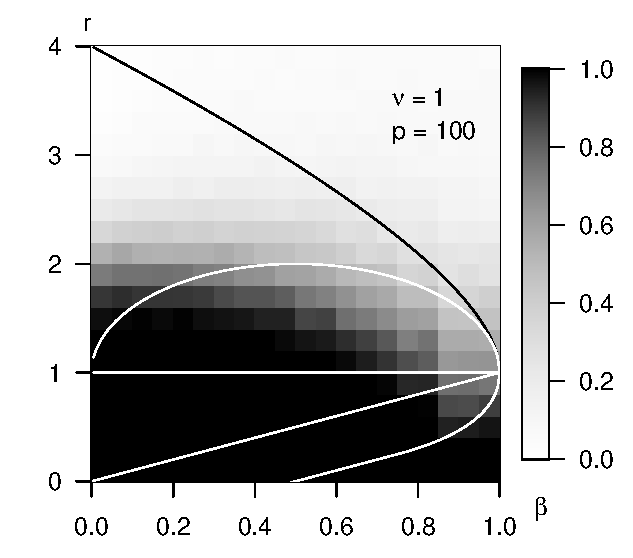
\includegraphics[width=0.32\textwidth]{./sim_approx-exact_boundary/simulated_approx-exact_boundary_chi-squared_nu1_p100.eps}
      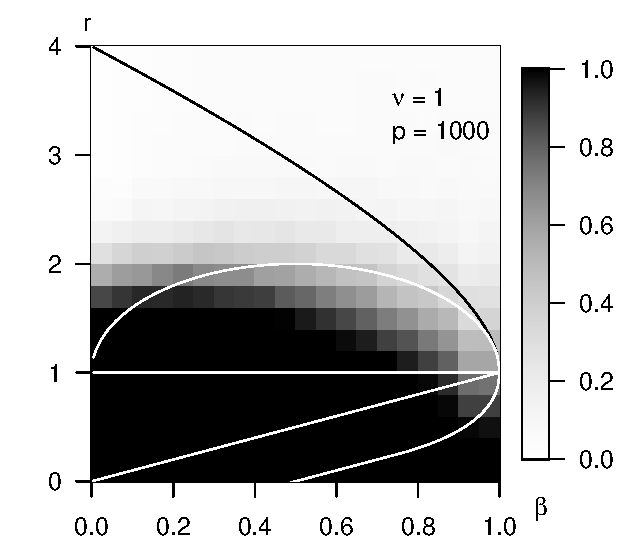
\includegraphics[width=0.32\textwidth]{./sim_approx-exact_boundary/simulated_approx-exact_boundary_chi-squared_nu1_p1000.eps}
      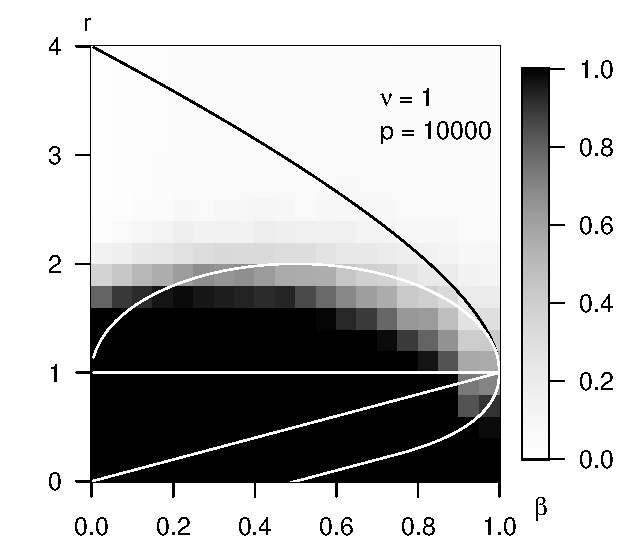
\includegraphics[width=0.32\textwidth]{./sim_approx-exact_boundary/simulated_approx-exact_boundary_chi-squared_nu1_p10000.eps}
      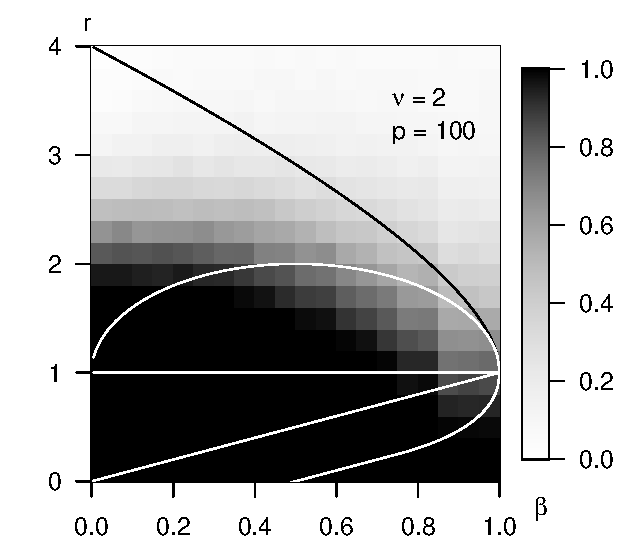
\includegraphics[width=0.32\textwidth]{./sim_approx-exact_boundary/simulated_approx-exact_boundary_chi-squared_nu2_p100.eps}
      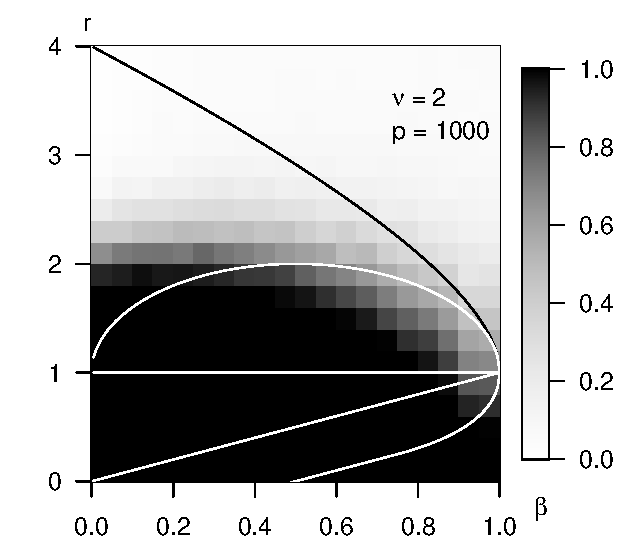
\includegraphics[width=0.32\textwidth]{./sim_approx-exact_boundary/simulated_approx-exact_boundary_chi-squared_nu2_p1000.eps}
      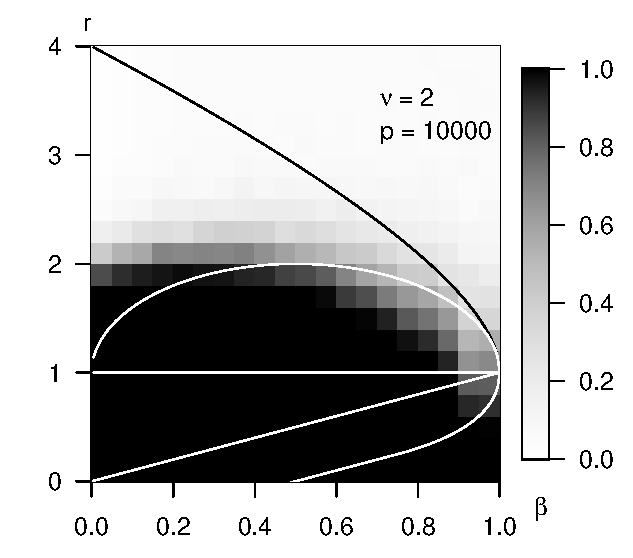
\includegraphics[width=0.32\textwidth]{./sim_approx-exact_boundary/simulated_approx-exact_boundary_chi-squared_nu2_p10000.eps}
      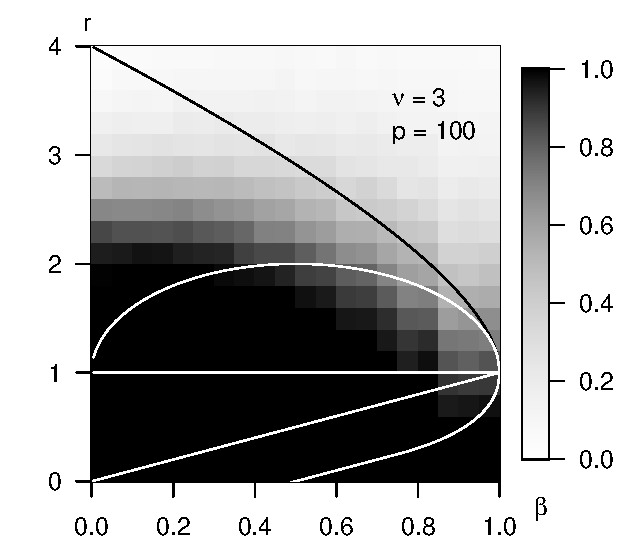
\includegraphics[width=0.32\textwidth]{./sim_approx-exact_boundary/simulated_approx-exact_boundary_chi-squared_nu3_p100.eps}
      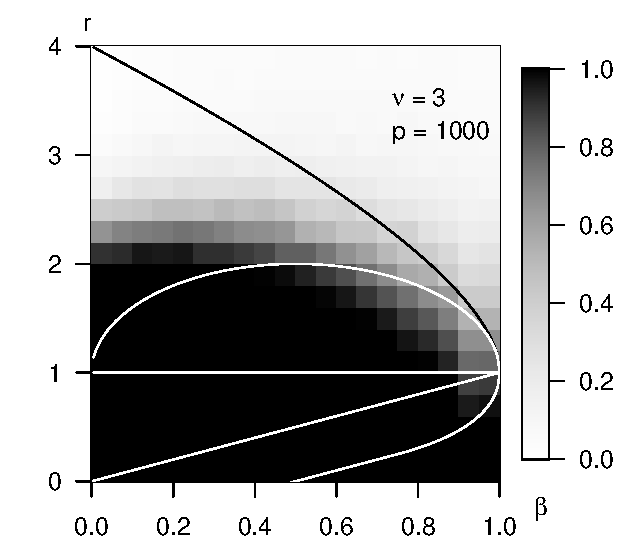
\includegraphics[width=0.32\textwidth]{./sim_approx-exact_boundary/simulated_approx-exact_boundary_chi-squared_nu3_p1000.eps}
      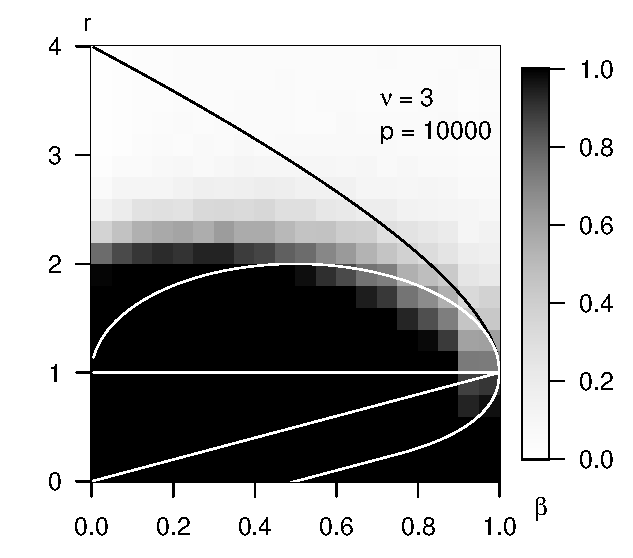
\includegraphics[width=0.32\textwidth]{./sim_approx-exact_boundary/simulated_approx-exact_boundary_chi-squared_nu3_p10000.eps}
      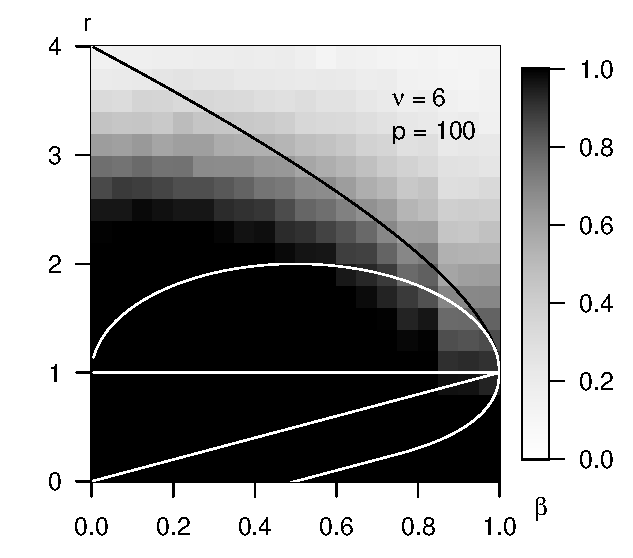
\includegraphics[width=0.32\textwidth]{./sim_approx-exact_boundary/simulated_approx-exact_boundary_chi-squared_nu6_p100.eps}
      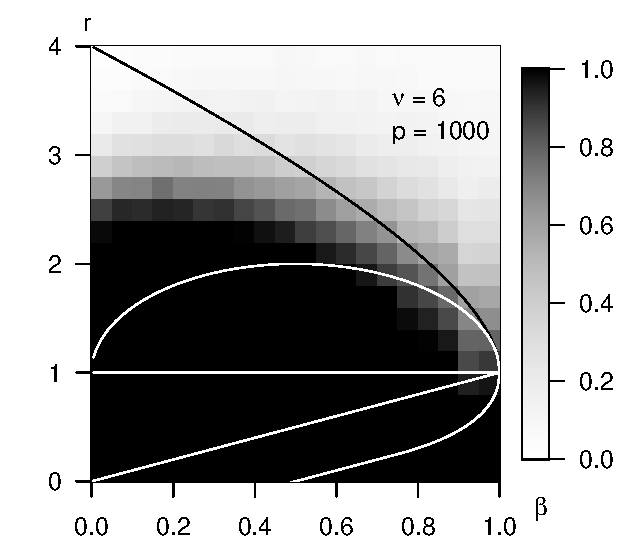
\includegraphics[width=0.32\textwidth]{./sim_approx-exact_boundary/simulated_approx-exact_boundary_chi-squared_nu6_p1000.eps}
      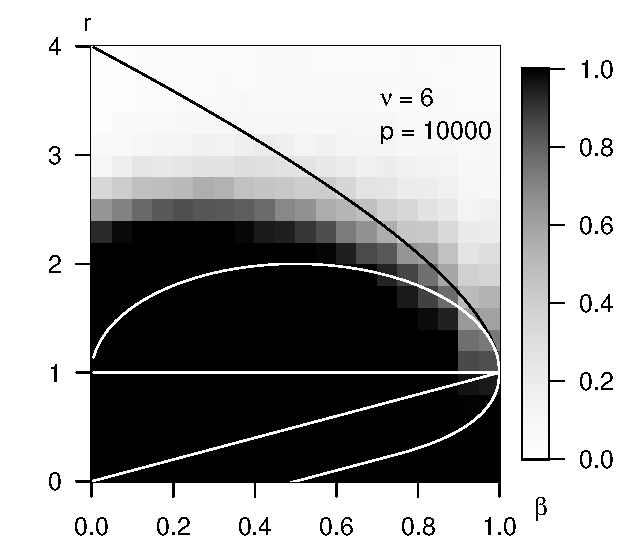
\includegraphics[width=0.32\textwidth]{./sim_approx-exact_boundary/simulated_approx-exact_boundary_chi-squared_nu6_p10000.eps}
      \caption{The estimated risk of approximate-exact support recovery $\mathrm{risk}^{\mathrm{EA}}$ (see \eqref{eq:risk-approx-exact}) of the Benjamini-Hochberg procedure in the chi-squared model \eqref{eq:model-chisq}. 
      We simulate $\nu=1, 2, 3, 6$ (first to last row), at dimensions $p=10^2, 10^3, 10^4$ (left to right column), for a grid of sparsity levels $\beta$ and signal sizes $r$.
      The experiments were repeated 1000 times for each sparsity-signal size combination; darker color indicates higher larger $\mathrm{risk}^{\mathrm{EA}}$. 
      Numerical results are generally in agreement with the boundaries described in Theorem \ref{thm:chi-squared-approx-boundary}; for small $\beta$'s and large $\nu$'s, the phase transitions take place somewhat above the predicted boundaries.
      Other boundaries in the support recovery and the detection problems are plotted for comparison.} 
      \label{fig:phase-simulated-chi-squared-approx-exact-boundary}
\end{figure}


\appendix
\section{Proofs}
\label{sec:proofs}


\subsection{Auxiliary facts about chi-square distributions}

We first establish some auxiliary facts about chi-square distributions, used in the proofs of Theorem \ref{thm:chi-squred-strong-boundary} and Theorem \ref{thm:chi-squred-weak-boundary}.

\begin{lemma}[Rapid variation of chi-square distribution tails] \label{lemma:rapid-variation-chisq}
The central chi-square distribution with $\nu$ degrees of freedom has rapidly varying tails.
That is, 
\begin{equation} \label{eq:rapid-variation-chisq}
    \lim_{x\to\infty}\frac{\P[\chi_\nu^2(0)>tx]}{\P[\chi_\nu^2(0)>x]} = 
    \begin{cases}
    0, & t > 1 \\
    1, & t = 1 \\
    \infty, & 0 < t < 1.
\end{cases}
\end{equation}
\end{lemma}

\begin{proof}[Proof of Lemma \ref{lemma:rapid-variation-chisq}]
When $\nu=1$, the chi-square distribution reduces to a squared Normal, and \eqref{eq:rapid-variation-chisq} follows from the rapid variation of the standard Normal distribution.
For $\nu\ge2$, we recall the following bound on tail probabilities (see, e.g., \citep{inglot2010inequalities}),
$$
\frac{1}{2}\mathcal{E}_\nu(x) \le \P[\chi_\nu^2(0)>x] \le \frac{x}{(x-\nu+2)\sqrt{\pi}} \mathcal{E}_\nu(x), \quad \nu\ge2,\;x>\nu-2,
$$
where $\mathcal{E}_\nu(x) = \exp\left\{-\frac{1}{2}[(x-\nu-(\nu-2)\log(x/\nu) + \log\nu]\right\}$.
Therefore, we have 
$$
\frac{(tx-\nu+2)\sqrt{\pi}}{2tx}\frac{\mathcal{E}_\nu(tx)}{\mathcal{E}_\nu(x)} 
\le \frac{\P[\chi_\nu^2(0)>tx]}{\P[\chi_\nu^2(0)>x]}
\le \frac{2tx}{(tx-\nu+2)\sqrt{\pi}}\frac{\mathcal{E}_\nu(tx)}{\mathcal{E}_\nu(x)},
$$
where ${\mathcal{E}_\nu(tx)}/{\mathcal{E}_\nu(x)} = \exp\{-\frac{1}{2}[(t-1)x-(\nu-2)\log{t}]\}$ converges to $0$ or $\infty$ depending on whether $t>1$ or $0<t<1$.
The case where $t=1$ is trivial.
\end{proof}

\begin{corollary} \label{cor:relative-stability}
Maxima of independent observations from central chi-square distributions with $\nu$ degrees of freedom are relatively stable. 
Specifically, let $\epsilon_p = \left(\epsilon_p(j)\right)_{j=1}^p$ be a i.i.d.\ $\chi_\nu^2(0)$. 
Define the sequence $(u_p)_{p=1}^\infty$ to be the $(1-1/p)$-th generalized quantiles, i.e., 
\begin{equation} \label{eq:quantiles}
    u_p = F^\leftarrow(1 - 1/p),
\end{equation}
where $F$ is the central chi-square distributions with $\nu$ degrees of freedom.
The triangular array ${\cal E} = \{\epsilon_p, p\in\N\}$ has relatively stable (RS) maxima, i.e.,
\begin{equation} \label{eq:RS-condition}
    \frac{1}{u_{p}} M_p := \frac{1}{u_{p}} \max_{j=1,\ldots,p} \epsilon_p(j) \xrightarrow{\P} 1,
\end{equation}
as $p\to\infty$.
\end{corollary}

\begin{proof}[Proof of Corollary \ref{cor:relative-stability}]
When $F(x)<1$ for all finite $x$, \citet{gnedenko1943distribution} showed that the distribution $F$ has rapidly varying tails if and only if the maxima of independent observations from $F$ are relatively stable.
Rapid variation follows from Lemma \ref{lemma:rapid-variation-chisq}.
\end{proof}


\begin{lemma}[Stochastic monotonicity] \label{lemma:stochastic-monotonicity}
The non-central chi-square distribution is stochastically monotone in its non-centrality parameter.
Specifically, for two non-central chi-square distributions both with $\nu$ degrees of freedom, and non-centrality parameters $\lambda_1 \le \lambda_2$, we have $\chi^2_\nu(\lambda_1) \stackrel{\mathrm{d}}{\le} \chi^2_\nu(\lambda_2)$. 
That is,
\begin{equation} \label{eq:stochastic-monotonicity}
    \P[\chi^2_\nu(\lambda_1) \le t] \ge \P[\chi^2_\nu(\lambda_2) \le t], \quad \text{for any}\quad t\ge0.
\end{equation}
\end{lemma}

\begin{proof}[Proof of Lemma \ref{lemma:stochastic-monotonicity}]
Recall that non-central chi-square distributions can be written as sums of $\nu-1$ standard normal random variables and a non-central normal random variable with mean $\sqrt{\lambda}$ and variance 1,
\begin{equation*}
    \chi_\nu^2(\lambda) 
    \stackrel{\mathrm{d}}{=} Z_1^2 + \ldots + Z_{\nu-1}^2 + (Z_\nu + \sqrt{\lambda})^2.
\end{equation*}
Therefore, it suffices to show that $\P[(Z+\sqrt{\lambda})^2 \le t]$ is non-increasing in $\lambda$ for any $t\ge0$, where $Z$ is a standard normal random variable.
We rewrite this expression in terms of standard normal probability function $\Phi$,
\begin{align}
    \P[(Z+\sqrt{\lambda})^2 \le t] 
    &= \P[-\sqrt{\lambda} - \sqrt{t} \le Z \le -\sqrt{\lambda} + \sqrt{t}] \nonumber \\
    &= \Phi(-\sqrt{\lambda} + \sqrt{t}) - \Phi(-\sqrt{\lambda} - \sqrt{t}). \label{eq:stochastic-monotonicity-proof-1}
\end{align}
The derivative of the last expression (with respect to $\lambda$) is 
\begin{equation} \label{eq:stochastic-monotonicity-proof-2}
    \frac{1}{2\sqrt{\lambda}} \left(\phi(\sqrt{\lambda} + \sqrt{t}) - \phi(\sqrt{\lambda} - \sqrt{t})\right) 
    = \frac{1}{2\sqrt{\lambda}} \left(\phi(\sqrt{\lambda} + \sqrt{t}) - \phi(\sqrt{t} - \sqrt{\lambda})\right),
\end{equation}
where $\phi$ is the density of the standard normal distribution.
Notice that we have used the symmetry of $\phi$ around 0 in the last expression.

Since $0 \le \max\{\sqrt{\lambda} - \sqrt{t}, \sqrt{t} - \sqrt{\lambda}\} < \sqrt{t} + \sqrt{\lambda}$ when $t>0$, by monotonicity of the normal density on $(0,\infty)$, we conclude that the derivative \eqref{eq:stochastic-monotonicity-proof-2} is indeed negative.
Therefore, \eqref{eq:stochastic-monotonicity-proof-1} is decreasing in $\lambda$, and \eqref{eq:stochastic-monotonicity} follows for $t>0$.
For $t = 0$, equality holds in \eqref{eq:stochastic-monotonicity} with both probabilities being 0.
\end{proof}


Finally, we derive asymptotic expressions for  chi-square quantiles.

\begin{lemma}[Chi-square quantiles] \label{lemma:chisq-quantiles}
Let $F$ be the central chi-square distributions with $\nu$ degrees of freedom, and let $u(y)$ be the $(1-y)$-th generalized quantile of $F$, i.e.,
\begin{equation} \label{eq:quantiles-generic}
    u(y) = F^\leftarrow(1 - y).
\end{equation}
Then 
\begin{equation}
    u(y) \sim 2\log(1/y), \quad \text{as }y\to0. 
\end{equation}
\end{lemma}

\begin{proof}[Proof of Lemma \ref{lemma:chisq-quantiles}]
The case where $\nu=1$ follows from the well-known Normal quantiles 
$$
F^\leftarrow(1 - 1/p) = \Phi^\leftarrow(1-1/(2p))\sim\sqrt{2\log{(2p)}}\sim\sqrt{2\log{p}}.
$$
The case where $\nu\ge2$ follows from the following estimates of high quantiles of chi-square distributions (see, e.g., \citep{inglot2010inequalities}),
$$
    \nu +  2\log(1/y) -5/2 \le u(y) \le \nu +  2\log(1/y) + 2\sqrt{\nu\log(1/y)}, \quad \text{for all }y\le0.17.
$$
\end{proof}


\subsection{Proof of Theorem \ref{thm:chi-squred-strong-boundary}}
\label{subsec:proof-chi-squred-strong-boundary}

\begin{proof}[Proof of Theorem \ref{thm:chi-squred-strong-boundary}]
We first prove the sufficient condition.
The condition $\underline{r} > {{g}}(\beta)$ implies, after some algebraic manipulation,
$\sqrt{\underline{r}} -\sqrt{1-\beta} > 1$.
Therefore, we can pick $q>1$ such that 
\begin{equation} \label{eq:choice-of-q}
    \sqrt{\underline{r}} -\sqrt{1-\beta} > \sqrt{q} > 1.
\end{equation}
The Bonferroni procedure sets the threshold at $t_p = F^\leftarrow(1-\alpha/p)$, which, by Lemma \ref{lemma:chisq-quantiles}, is asymptotic to $2\log{p} - 2\log{\alpha}$.
By the assumption on $\alpha$ in \eqref{eq:slowly-vanishing-error}, for any $\delta>0$, we have $\alpha\gg p^{-\delta}$ for large $p$.
Therefore, $-\log\alpha\ll\delta\log{p}$ eventually, and we have
$$
1 \le \limsup_{p\to\infty}\frac{2\log{p} - 2\log{\alpha}}{2\log{p}} \le 1+\delta,
$$
for any $\delta>0$.
Hence, $t_p\sim 2\log{p}$.
Setting the $t^* = t^*_p = 2q\log{p}$, we have $t_p < t^*_p$ for large $p$.


On the one hand, $\text{FWER} = 1 - \P[\widehat{S}_p \subseteq S_p]$ vanishes under the Bonferroni procedure with $\alpha\to0$.
On the other hand, for large $p$, the probability of no missed detection is bounded from below by
\begin{equation} \label{eq:chi-square-sufficient-1}
    \P[\widehat{S}_p \supseteq S_p] 
    = \P[\min_{i\in S} x(i) \ge t_p] 
    \ge \P[\min_{i\in S} x(i) \ge t^*] 
    \ge 1 - p^{1-\beta}\P[\chi_\nu^2(\underline{\Delta}) \le t^*],
\end{equation}
where we have used the fact that signal sizes are bounded below by $\underline{\Delta}$, and the stochastic monotonicity of chi-square distributions (Lemma \ref{lemma:stochastic-monotonicity}) in the last inequality.
Writing
$$
\chi_\nu^2(\underline{\Delta}) \stackrel{\mathrm{d}}{=} Z_1^2 + \ldots + Z_{\nu-1}^2 + (Z_\nu + \sqrt{\underline{\Delta}})^2
$$
where $Z_i$'s are iid standard normal variables, we have
\begin{align}
    \P[\chi_\nu^2({\underline{\Delta}}) \le t^*]
    &\le \P[(Z_\nu+\sqrt{\underline{\Delta}})^2 \le t^*] 
    = \P[|Z_\nu+\sqrt{\underline{\Delta}}| \le \sqrt{t^*}]  \nonumber \\
    &\le \P\left[Z_\nu \le - \sqrt{\underline{\Delta}} +  \sqrt{t^*}\right] \nonumber \\
    &= \P\left[Z_\nu \le \sqrt{2\underline{r}\log{p}}\left(\sqrt{q} - \sqrt{\underline{r}}\right)\right]. \label{eq:chi-square-sufficient-2}
\end{align}
By our choice of $q$ in \eqref{eq:choice-of-q}, the last probability in \eqref{eq:chi-square-sufficient-2}
is bounded above by 
$$
\P\Big[Z_\nu \le -\sqrt{2(1-\beta)\log{p}}\Big] = o\left(p^{-(1-\beta)}\right).
$$
This, combined with \eqref{eq:chi-square-sufficient-1}, completes the proof of the sufficient condition for the Bonferroni's procedure.

Under the assumption of independence, Sid\'ak's, Holm's, and Hochberg's procedures are strictly more powerful than Bonferroni's procedure, while controlling FWER at the nominal levels.
Therefore, the risks of exact support recovery for these procedures also vanishes.
This completes the proof for the first part of Theorem \ref{thm:chi-squred-strong-boundary}.

We now show the necessary condition. 
We first normalize the maxima by the chi-square quantiles $u_p = F^{\leftarrow}(1-1/p)$, where $F$ is the distribution of a (central) chi-square random variable,
\begin{equation} \label{eq:chi-square-necessary-0}
 \P[\widehat{S}_p = S_p] \le \P\left[\max_{i\in S^c}x(i) < \min_{i\in S}x(i)\right]
  % &= \P\left[\frac{\max_{i\in S^c}x(i)}{u_p} < \frac{\min_{i\in S}x(i)}{u_p}\right] \nonumber \\
  % &\le  \P\left[\frac{\max_{i\in S^c}\chi_\nu^2(\lambda(i))}{u_p} < \frac{\min_{i\in S}\chi_\nu^2(\lambda(i))}{u_p}\right] \nonumber \\
  = \P\left[ \frac{M_{S^c}}{u_p} < \frac{m_S}{u_p} \right],
\end{equation}
where $M_{S^c} = \max_{i\in S^c}\chi_\nu^2(\lambda(i))$ and $m_{S} = \min_{i\in S}\chi_\nu^2(\lambda(i))$.
Writing
\begin{equation} \label{eq:chi-square-necessary-1}
    \frac{M_{S^c}}{u_{p}} = \frac{M_{S^c}}{u_{p-p^{1-\beta}}} \frac{u_{p-p^{1-\beta}}}{u_{p}}, % \stackrel{\P}{\longrightarrow} 1,
\end{equation}
we know by the relative stability of chi-square random variables (Corollary \ref{cor:relative-stability}) that the first term in the product converges to 1 in probability.
The second term, using the expression for chi-square quantiles (Lemma \ref{lemma:chisq-quantiles}), is asymptotic to 
$$
\frac{2\log{(p-p^{1-\beta})}}{2\log{p}} = \frac{\log{p}+\log{(1-p^{-\beta})}}{\log{p}} \sim 1.
$$
Therefore, the expression \eqref{eq:chi-square-necessary-1} converges to $1$ in probability.

Meanwhile, for any $i\in S$, by Lemma \ref{lemma:stochastic-monotonicity} and the fact that signal sizes are bounded above by $\overline{\Delta}$, we have,
\begin{equation*}
    {\chi_\nu^2(\lambda(i))} \stackrel{\mathrm{d}}{\le}
    {\chi_\nu^2(\overline{\Delta})} \stackrel{\mathrm{d}}{=} 
    {Z_1^2 + \ldots + Z_{\nu-1}^2 + \left(Z_\nu + \sqrt{\overline{\Delta}}\right)^2}.
\end{equation*}
Dividing through by $u_p$, and taking minimum over $S$, we obtain
\begin{equation} \label{eq:chi-square-necessary-3}
    \frac{m_S}{u_p} 
    = \min_{i\in S} \frac{\chi_\nu^2(\lambda(i))}{u_p} 
    % \stackrel{\mathrm{d}}{\le} \min \left\{\frac{\chi_\nu^2(\overline{\Delta})}{u_p}, s \text{ i.i.d. copies} \right\} \\
    \stackrel{\mathrm{d}}{\le} \min_{i\in S}\frac{Z_1^2(i) + \ldots + Z_{\nu-1}^2(i)}{u_p} + \frac{(Z_\nu(i) + \sqrt{\overline{\Delta}})^2}{u_p}.
\end{equation}
Let $i^\dagger = i^\dagger_p$ be the index minimizing the second term in \eqref{eq:chi-square-necessary-3}, i.e.,
\begin{equation}
    i^\dagger := \argmin_{i\in S} \frac{(Z_\nu(i) + \sqrt{\overline{\Delta}})^2}{u_p}
    = \argmin_{i\in S} \frac{(Z_\nu(i) + \sqrt{\overline{\Delta}})^2}{2\log{p}},
\end{equation}
and define the function $f_p(x):=(x+\sqrt{\overline{\Delta}})^2/(2\log{p})$, we shall first show that 
\begin{equation} \label{eq:chi-square-necessary-4}
    %\min_{i\in S} \frac{(Z_\nu(i) + \sqrt{\overline{\Delta}})^2}{2\log{p}} 
    \P[ f_p(Z_\nu(i^\dagger)) < 1 ] \to 1.
\end{equation}
On the one hand, we know (by solving a quadratic inequality) that
\begin{equation} \label{eq:chi-square-necessary-5}
    f_p(x)<1 \iff \frac{x}{\sqrt{2\log{p}}} \in (-(\sqrt{\overline{r}}+1), -(\sqrt{\overline{r}}-1)).
\end{equation}
On the other hand, we know (by relative stability of i.i.d. Gaussians) that 
\begin{equation} \label{eq:chi-square-necessary-6}
    \frac{\min_{i\in S} Z_\nu(i)}{\sqrt{2\log{p}}}
    \to -\sqrt{1-\beta} \quad\text{in probability}.
\end{equation}
Further, by the assumption on the signal sizes $\overline{r} < (1+\sqrt{1-\beta})^2$, we have,
\begin{equation} \label{eq:chi-square-necessary-7}
    -(\sqrt{\overline{r}}+1) < - \sqrt{1-\beta} < - (\sqrt{\overline{r}}-1).
\end{equation}
Combining \eqref{eq:chi-square-necessary-5}, \eqref{eq:chi-square-necessary-6}, and \eqref{eq:chi-square-necessary-7}, we obtain
$$
\P\left[ f_p(Z_\nu(i^\dagger)) < 1 \right] \ge \P\left[ f_p\left(\min_{i\in S}Z_nu(i)\right) < 1 \right] \to 1,
$$
and we arrive at \eqref{eq:chi-square-necessary-4}.
As a corollary, since $u_p\sim2\log{p}$,
\begin{equation} \label{eq:chi-square-necessary-8}
    \P\left[\frac{(Z_\nu(i) + \sqrt{\overline{\Delta}})^2}{u_p} < 1\right]\to1.
\end{equation}

Finally, by independence between $Z_1^2(i)+\ldots+Z_{\nu-1}^2(i)$ and $(z_\nu^2(i)+\sqrt{\overline{\Delta}})^2$, and the fact that $i^\dagger$ is a function of only the second term, we have
$$
Z_1^2(i^\dagger)+\ldots+Z_{\nu-1}^2(i^\dagger) 
\stackrel{\mathrm{d}}{=} Z_1^2(i)+\ldots+Z_{\nu-1}^2(i) 
\quad \text{for all} \;\; i\in S.
$$
Therefore, $Z_1^2(i^\dagger)+\ldots+Z_{\nu-1}^2(i^\dagger) = O_\P(1)$, and 
\begin{equation} \label{eq:chi-square-necessary-9}
    \frac{Z_1^2(i^\dagger)+\ldots+Z_{\nu-1}^2(i^\dagger)}{u_p} \to 0 \quad \text{in probability}. 
\end{equation}
Together, \eqref{eq:chi-square-necessary-8} and \eqref{eq:chi-square-necessary-9} implies that
\begin{align}
    \P\left[\frac{m_S}{u_p}<1\right]
    &\ge \P\left[\min_{i\in S}\frac{Z_1^2(i) + \ldots + Z_{\nu-1}^2(i)}{u_p} + \frac{(Z_\nu(i) + \sqrt{\overline{\Delta}})^2}{u_p} < 1\right] \nonumber \\
    &\ge \P\left[\frac{Z_1^2(i^\dagger) + \ldots + Z_{\nu-1}^2(i^\dagger)}{u_p} + \frac{(Z_\nu(i^\dagger) + \sqrt{\overline{\Delta}})^2}{u_p} < 1\right] \to 1. \label{eq:chi-square-necessary-10}
\end{align}
In view of \eqref{eq:chi-square-necessary-0}, \eqref{eq:chi-square-necessary-1}, and \eqref{eq:chi-square-necessary-10}, we conclude that exact recovery cannot succeed with any positive probability.
The proof of the necessary condition is complete.
\end{proof}

\subsection{Proof of Theorem \ref{thm:chi-squred-weak-boundary}}
\label{subsec:proof-chi-squred-weak-boundary}

We first show the necessary condition. 
That is, when $\overline{r} < \beta$, no thresholding procedure is able to achieve approximate support recovery.
The main structure of the proof follows that of Theorem 1 in \citet{arias2017distribution}. 
Our arguments, however, allow for unequal signal sizes; these arguments can in turn be used to generalize the results in \cite{arias2017distribution}.

\begin{proof}[Proof of necessary condition in Theorem \ref{thm:chi-squred-weak-boundary}]
Denote the distributions of $\chi^2_\nu(0)$, $\chi^2_\nu(\underline{\Delta})$ and $\chi^2_\nu(\overline{\Delta})$ as $F_0$, $F_{\underline{a}}$, and $F_{\overline{a}}$ respectively.

We first show the necessary condition, i.e., when $\overline{r}<\beta$, approximate support recovery cannot be achieved with any thresholding procedure.
In particular, we show that the liminf of the sum of FDP and NDP is at least 1.

Recall that thresholding procedures are of the form
$$
\widehat{S}_p = \left\{i\,|\,x(i) > t_p(x)\right\}.
$$
Denote $\widehat{S} := \left\{i\,|\,x(i) > t_p(x)\right\}$, and $\widehat{S}(u) := \left\{i\,|\,x(i) > u\right\}$.
For any threshold $u\ge t_p$ we must have $\widehat{S}(u)\subseteq\widehat{S}$, and hence
\begin{equation} \label{eq:weak-boundary-proof-FDP}
    \text{FDP} = \frac{|\widehat{S}\setminus{S}|}{|\widehat{S}|} \ge \frac{|\widehat{S}\setminus{S}|}{|\widehat{S}\cup{S}|} = \frac{|\widehat{S}\setminus{S}|}{|\widehat{S}\setminus{S}| + |S|} \ge
    \frac{|\widehat{S}(u)\setminus{S}|}{|\widehat{S}(u)\setminus{S}| + |S|}.
\end{equation}
On the other hand, for any threshold $u\le t_p$ we must have $\widehat{S}(u)\supseteq\widehat{S}$, and hence
\begin{equation} \label{eq:weak-boundary-proof-NDP}
    \text{NDP} = \frac{|{S}\setminus\widehat{S}|}{|{S}|} \ge 
    \frac{|{S}\setminus\widehat{S}(u)|}{|{S}|}.
\end{equation}
Since either $u\ge t_p$ or  $u\le t_p$ must take place, putting \eqref{eq:weak-boundary-proof-FDP} and \eqref{eq:weak-boundary-proof-NDP} together, we have
\begin{equation} \label{eq:weak-boundary-proof-converse-1}
    \text{FDP} + \text{NDP} 
    \ge \frac{|\widehat{S}(u)\setminus{S}|}{|\widehat{S}(u)\setminus{S}|+|{S}|} \wedge \frac{|{S}\setminus\widehat{S}(u)|}{|{S}|},
\end{equation}
for any $u$.
Therefore it suffices to show that for a suitable choice of $u$, the RHS of \eqref{eq:weak-boundary-proof-converse-1} converges to 1.

Let $t^* = 2q\log{p}$, where $\overline{r}<q<\beta$, we obtain an estimate of the tail probability
\begin{align}
    \overline{F_0}(t^*) 
    &= \P[\chi_\nu^2(0) > t^*] 
    = \frac{2^{1-\nu/2}}{\Gamma(\nu/2)} \int_{2q\log{p}}^\infty x^{\nu/2-1}e^{-x/2} \mathrm{d}x \nonumber \\
    &\sim \frac{2^{1-\nu/2}}{\Gamma(\nu/2)} \left(2q\log{p}\right)^{\nu/2-1}p^{-q}, \label{eq:weak-boundary-proof-null-tail-prob}
\end{align}
where $a_p\sim b_p$ is taken to mean $a_p/b_p\to 1$.
Observe that $|\widehat{S}(t^*)\setminus{S}|$ has distribution $\text{Binom}(p-s, \overline{F_0}(t^*))$, denote $X = X_p := {|\widehat{S}(t^*)\setminus{S}|}/{|S|}$, and we have 
$$
\mu := \E\left[X\right] = \frac{(p-s)\overline{F_0}(t^*)}{s},
\quad \text{and} \quad
\var\left(X\right) = \frac{(p-s)\overline{F_0}(t^*){F_0}(t^*)}{s^2} \le \mu/s.
$$
Therefore for any $M>0$, we have, by Chebyshev's inequality,
\begin{equation}
    \P\left[X < M\right] 
    \le \P\left[\left|X-\mu\right| > \mu - M\right]
    \le \frac{\mu/s}{(\mu-M)^2}
    = \frac{1/(\mu s)}{(1-M/\mu)^2}. \label{eq:weak-boundary-proof-converse-2}
\end{equation}
Now, from the expression of $\overline{F_0}(t^*)$ in \eqref{eq:weak-boundary-proof-null-tail-prob}, we obtain
$$
\mu = (p^\beta - 1)\overline{F_0}(t^*) \sim \frac{2^{1-\nu/2}}{\Gamma(\nu/2)} \left(2q\log{p}\right)^{\nu/2-1}p^{\beta-q}\to\infty \quad \text{ as }\;p\to\infty.
$$
Therefore the last expression in \eqref{eq:weak-boundary-proof-converse-2} converges to 0, and we conclude that $X\to\infty$ in probability, and hence
$$
\frac{|\widehat{S}(t^*)\setminus{S}|}{|\widehat{S}(t^*)\setminus{S}|+|{S}|} 
= \frac{X}{X+1} \to 1 \quad \text{in probability}.
$$

On the other hand, we show that with the same choice of $u = t^*$,
$$
\frac{|{S}\setminus\widehat{S}(t^*)|}{|{S}|}\to 1 \quad \text{in probability}.
$$
By the stochastic monotonicity of chi-square distributions (Lemma \ref{lemma:stochastic-monotonicity}), the probability of missed detection for each signal is lower bounded by $\P[\chi^2_\nu(\lambda_i) \le t^*] \ge F_{\overline{a}}(t^*))$.
Therefore, $|{S}\setminus\widehat{S}(t^*)| \stackrel{\mathrm{d}}{\ge} \text{Binom}(s, {F_{\overline{a}}}(t^*))$, and it suffices to show that ${F_{\overline{a}}}(t^*)$ converges to 1.
This is indeed the case, since
\begin{align*}
    {F_{\overline{a}}}(t^*) 
    &= \P[Z_1^2 + \ldots + Z_\nu^2 + 2\sqrt{2\overline{r}\log{p}} Z_\nu + 2\overline{r}\log{p} \le 2q\log{p}] \\
    &\ge \P[Z_1^2 + \ldots + Z_\nu^2 \le (q-\overline{r})\log{p}, \; 2\sqrt{2\overline{r}\log{p}} Z_\nu \le (q-\overline{r})\log{p}],
\end{align*}
and both events in the last line have probability going to 1 as $p\to\infty$.
The necessary condition is shown.
\end{proof}

We now turn to the sufficient condition. 
That is, when $\underline{r} > \beta$, the Benjamini-Hochberg procedure with slowly vanishing FDR levels achieves asymptotic approximate support recovery.

The proof proceeds in two steps.
We first make the connection between power of the BH procedure and stochastic ordering of the alternatives.
It is formalized in the following lemma, which could be of independent interest.
This result, though natural, seems new. 

\begin{lemma}[Monotonicity of the BH procedure] \label{lemma:monotonicity-BH-procedure}
Compare Alternatives 1 and 2 where we have $p$ independent observations $x(i)$, $i\in\{1,\ldots,p\}$,
\begin{enumerate}
    \item[Alt.1] the $p-s$ coordinates in the null part have common distribution $F_0$, and the $s$ signals have alternative distributions $F^{i}_1$, $i\in S$, respectively.
    \item[Alt.2] the $p-s$ coordinates in the null part have common distribution $F_0$, and the $s$ signals have alternative distributions $F^{i}_2$, $i\in S$, respectively, where
    $$ F^{i}_2(t) \le F^{i}_1(t), \quad \text{for all} \;\; t\in\R, \; \text{and for all} \;\; i\in S.$$
\end{enumerate}
If we apply the BH procedure at the same nominal level of FDR $\alpha$, then the FNR under Alternative 2 is bounded above by the FNR under Alternative 1.
\end{lemma}

Loosely put, the power of the BH procedure is monotone increasing with respect to the stochastic ordering of the alternatives.

\begin{proof}[Proof of Lemma \ref{lemma:monotonicity-BH-procedure}]
We first re-express the BH procedure in a different form.
Recall that on observing $x(i)$, $i\in\{1,\ldots,p\}$, the BH procedure is the thresholding procedure with threshold set at $x_{[i^*]}$, where $i^* := \max\{i\,|\,\overline{F_0}(x_{[i]})\le \alpha i/p\}$, and $x_{[1]}\ge\ldots\ge x_{[p]}$ are the order statistics.

Let $\widehat{G}$ denote the empirical survival function
\begin{equation} \label{eq:empirical-tail-distribution}
    \widehat{G}(t) = \frac{1}{p}\sum_{i\in[p]}\mathbbm{1}\{x(i) \ge t\}.
\end{equation}
By the definition, we know that $\widehat{G}(x_{[i]}) = i/p$.
Therefore, by the definition of $i^*$, we have
\begin{equation*} 
    \overline{F_0}(x_{[i]}) > \alpha\widehat{G}(x_{[i]}) = \alpha i/p \quad \text{for all }i>i^*.
\end{equation*}
Since $\widehat{G}$ is constant on $(x_{[i^*+1]}, x_{[i^*]}]$, the fact that 
$\overline{F_0}(x_{[i^*]}) \le \alpha\widehat{G}(x_{[i^*]})$ and $\overline{F_0}(x_{[i^*+1]}) > \alpha\widehat{G}(x_{[i^*+1]})$ implies that $\alpha\widehat{G}$ and $\overline{F_0}$ must ``intersect'' on the interval.
We denote this ``intersection'' as
\begin{equation} \label{eq:weak-boundary-proof-tau}
    \tau = \inf\{t\,|\,\overline{F_0}(t)\le\alpha\widehat{G}(t)\}. 
    %= \min\{t\,|\,\overline{F_0}(t)=\alpha\widehat{G}(t)\}.
\end{equation}
Note that $\tau$ cannot be equal to $x_{[i^*+1]}$ since $\overline{F}_0$ is C\`adl\`ag.
Since there is no observation in $[\tau, x_{[i^*]})$, we can write the BH procedure as the thresholding procedure with threshold set at $\tau$.

Now, denote the observations under Alternatives 1 and 2 as $x_1(i)$ and $x_2(i)$.
Since $x_2(i)$ stochastically dominates $x_1(i)$ for all $i\in\{1,\ldots,p\}$, there exists a coupling $(\widetilde{x}_1, \widetilde{x}_2)$ of $x_1$ and $x_2$ such that 
% $\widetilde{x}_1(i) = \widetilde{x}_2(i)$ for $i\in S^c$, and 
$\widetilde{x}_1(i) \le \widetilde{x}_2(i)$ a.s. for all $i$.
We will replace $x_1$ and $x_2$ with $\widetilde{x}_1$ and $\widetilde{x}_2$ in what follows.
Since we will compare expectations with respect to $\widetilde{x}$'s in the last step, this replacement does not cause any trouble.
To simplify notation, we still write $x_1$ and $x_2$ in place of $\widetilde{x}_1$ and $\widetilde{x}_2$.

Let $\widehat{G}_k$ be the empirical survival function under Alternative $k$, i.e.,
\begin{equation} \label{eq:empirical-survival}
    \widehat{G}_k(t) = \frac{1}{p}\sum_{i\in[p]}\mathbbm{1}\{x_k(i) \ge t\}, \quad k\in\{1,2\}.
\end{equation}
We define the BH thresholds $\tau_1$ and $\tau_2$ by replacing $\widehat{G}$ in \eqref{eq:weak-boundary-proof-tau} with $\widehat{G}_1$ and $\widehat{G}_2$, respectively.
Denote the set estimates of signal support $\widehat{S}_k = \{i\,|\,x_k(i)\ge\tau_k\}$ by the BH procedure.
We claim that (perhaps surprisingly),
\begin{equation} \label{eq:monotonicity-BH-procedure-thresholds}
    \tau_2 \le \tau_1 \quad \text{with probability } 1.
\end{equation}

Indeed, by definition of the empirical survival function \eqref{eq:empirical-survival} and the fact that $x_1(i) \le x_2(i)$ almost surely for all $i$,  we have $\widehat{G}_1(t) \le \widehat{G}_2(t)$ for all $t$.
Hence, $\overline{F_0}(t)\le\alpha\widehat{G}_1(t)$ implies $\overline{F_0}(t)\le\alpha\widehat{G}_2(t)$, and Relation \eqref{eq:monotonicity-BH-procedure-thresholds} follows from the definition of $\tau$ in \eqref{eq:weak-boundary-proof-tau}.

Finally, when $\tau_2 \le \tau_1$, we have $\tau_2 \le \tau_1 \le x_1(i) \le x_2(i)$ with probability 1 for all $i\in\widehat{S}_1$.
Therefore, it follows that $\widehat{S}_1 \subseteq \widehat{S}_2$ and hence $|S\setminus\widehat{S}_2| \le |S\setminus\widehat{S}_1|$ almost surely. 
The conclusion in Lemma \ref{lemma:monotonicity-BH-procedure} follows from the last inequality.
\end{proof}

Lemma \ref{lemma:monotonicity-BH-procedure} allows us to reduce the alternative with unequal signal sizes to one with equal signal sizes in the proof of the sufficient condition. 

\begin{proof}[Proof of sufficient condition in Theorem \ref{thm:chi-squred-weak-boundary}]
The FDR vanishes by our choice of $\alpha$ and the FDR-controlling property of the BH procedure.
It only remains to show that FNR also vanishes.

To do so we compare the FNR under the alternative specified in Theorem \ref{thm:chi-squred-weak-boundary} to one with all of the signal sizes equal to $\underline{\Delta}$.
Let $x(i)$ be vectors of independent observations with $p-s$ nulls having $\chi^2_\nu(0)$ distributions, and $s$ signals having $\chi^2_\nu(\underline{\Delta})$ distributions.
By Lemma \ref{lemma:stochastic-monotonicity} Lemma \ref{lemma:monotonicity-BH-procedure}, it suffices to show that the FNR under the BH procedure in this setting vanishes.

Let $\widehat{G}$ denote the empirical survival function as in \eqref{eq:empirical-tail-distribution}.
Define the empirical survival functions for the null part and signal part
\begin{equation} \label{eq:empirical-survival-null-signal}
    \widehat{W}_\text{null}(t) = \frac{1}{p-s}\sum_{i\not\in S}\mathbbm{1}\{x(i) \ge t\},
    \quad
    \widehat{W}_\text{signal}(t) = \frac{1}{s}\sum_{i\in S}\mathbbm{1}\{x(i) \ge t\},
\end{equation}
so that
$$
\widehat{G}(t) = \frac{p-s}{p}\widehat{W}_\text{null}(t) + \frac{s}{p}\widehat{W}_\text{signal}(t).
$$

We need the following result to describe the deviations of the empirical distributions.
\begin{lemma}[\cite{eicker1979asymptotic}] \label{lemma:empirical-process}
Let $Z_1,\ldots,Z_k$ be i.i.d.\ with continuous survival function $Q$.
Let $\widehat{Q}_k$ denote their empirical survival function and define 
$\xi_k = \sqrt{2\log{\log{(k)}}/k}$ for $k \ge 3$. 
Then
$$
\frac{1}{\xi_k}\sup_z\frac{\widehat{Q}_k(z) - Q(z)}{\sqrt{Q(z)(1 - Q(z))}} \to 1,
$$
in probability as $k \to \infty$.
In particular,
$$
\widehat{Q}_k(z) = Q(z) + O_\P\left(\xi_k\sqrt{Q(z)(1 - Q(z))}\right),
$$
uniformly in z.
\end{lemma}

Apply Lemma \ref{lemma:empirical-process} to $\widehat{G}$, we obtain
$\widehat{G}(t) = G(t) + \widehat{R}(t)$.
where 
\begin{equation} \label{eq:empirical-process-mean}
    G(t) = \frac{p-s}{p}\overline{F_0}(t) + \frac{s}{p}\overline{F_a}(t),
\end{equation}
where $\overline{F_0}$ and $\overline{F_{a}}$ are the survival functions of $\chi_\nu^2(0)$ and $\chi_\nu^2(\underline{\Delta})$ respectively, and 
\begin{equation} \label{eq:empirical-process-residual}
    \widehat{R}(t) = O_\P\left(\xi_p\sqrt{\overline{F_0}(t)F_0(t)} + \frac{s}{p}\xi_s\sqrt{\overline{F_a}(t)F_a(t)}\right),
\end{equation}
uniformly in $t$.

Recall (see proof of Lemma \ref{lemma:monotonicity-BH-procedure}) that the BH procedure is the thresholding procedure with threshold set at $\tau$ (defined in \eqref{eq:weak-boundary-proof-tau}).
% \begin{equation} \label{eq:weak-boundary-proof-tau-recall}
%     \tau = \inf\{t\,|\,\overline{F_0}(t)\le\alpha\widehat{G}(t)\}. 
%     %= \min\{t\,|\,\overline{F_0}(t)=\alpha\widehat{G}(t)\}.
% \end{equation}
The NDP may also be re-written as 
$$
\text{NDP} = \frac{|{S}\setminus\widehat{S}|}{|{S}|} = \frac{1}{s}\sum_{i\in S}\mathbbm{1}\{x(i) < \tau\} = 1 - \widehat{W}_\text{signal}(\tau),
$$
so that it suffices to show that 
\begin{equation} \label{eq:weak-boundary-proof-sufficient-1}
    \widehat{W}_\text{signal}(\tau)\to 1
\end{equation} in probability.
Applying Lemma \ref{lemma:empirical-process} to $\widehat{W}_\text{signal}$, we know that 
$$
\widehat{W}_\text{signal}(\tau) = \overline{F_a}(\tau) + O_\P\left(\xi_s\sqrt{\overline{F_a}(\tau)F_a(\tau)}\right) = \overline{F_a}(\tau) + o_\P(1).
$$
So it suffices to show that $F_a(\tau)\to 0$ in probability.
Now let $t^* = 2q\log(p)$ for some $q$ such that $\beta<q<r$.
We have 
\begin{equation} \label{eq:weak-boundary-proof-sufficient-2}
    F_a(t^*) = \P[\chi^2_\nu(\underline{\Delta}) \le t^*]
    \le \P\left[2\sqrt{\underline{\Delta}}Z_\nu \le t^* - \underline{\Delta}\right] 
    = \P\left[Z_\nu \le \frac{t^*}{2\sqrt{\underline{\Delta}}} - \frac{\sqrt{\underline{\Delta}}}{2}\right] \to 0.
\end{equation}
Hence in order to show \eqref{eq:weak-boundary-proof-sufficient-1}, it suffices to show 
\begin{equation} \label{eq:weak-boundary-proof-sufficient-3}
    \P\left[\tau \le t^*\right] \to 1.
\end{equation}
By \eqref{eq:empirical-process-mean}, the mean of the empirical process $\widehat{G}$ evaluated at $t^*$ is
\begin{equation*}
    G(t^*) = \frac{p-s}{p}\overline{F_0}(t^*) + \frac{s}{p}\overline{F_a}(t^*).
\end{equation*}
The first term, using Relation \eqref{eq:weak-boundary-proof-null-tail-prob}, is asymptotic to $p^{-q}L(p)$, where $L(p)$ is the logarithmic term in $p$.
The second term, since $\overline{F_a}(t^*)\to 1$ by Relation \eqref{eq:weak-boundary-proof-sufficient-2}, is asymptotic to $p^{-\beta}$.
Therefore, $G(t^*) \sim p^{-q}L(p) + p^{-\beta} \sim p^{-\beta}$, since $q>\beta$ and $p^\delta L(p)$ for all $\delta>0$.

The fluctuation of the empirical process at $t^*$, by Relation \eqref{eq:empirical-process-residual}, is 
\begin{align*}
    \widehat{R}(t^*) 
    &= O_\P\left(\xi_p\sqrt{\overline{F_0}(t^*)F_0(t^*)} + \frac{s}{p}\xi_s\sqrt{\overline{F_a}(t^*)F_a(t^*)}\right)\\
    &= O_\P\left(\xi_p\sqrt{\overline{F_0}(t^*)}\right) + o_\P\left(p^{-\beta}\right).
\end{align*}
By \eqref{eq:weak-boundary-proof-null-tail-prob} and the expression for $\xi_p$, the first term is $O_\P\left(p^{-(q+1)/2}L(p)\right)$ where $L(p)$ is a poly-logarithmic term in $p$.
Since $\beta<\min\{q,1\}$, we have $\beta<(q+1)/2$, and hence $\widehat{R}(t^*) = o_\P(p^{-\beta})$.

Putting the mean and the fluctuation of $\widehat{G}(t^*)$ together, we obtain
$$
\widehat{G}(t^*) = G(t^*) + \widehat{R}(t^*) \sim_\P G(t^*) \sim p^{-\beta},
$$
and therefore, together with \eqref{eq:weak-boundary-proof-null-tail-prob}, we have
$$
\overline{F_0}(t^*)/\widehat{G}(t^*) = p^{\beta-q}L(p)(1+o_{\P}(1)),
$$
which is eventually smaller than the FDR level $\alpha$ by the assumption \eqref{eq:slowly-vanishing-error} and the fact that $\beta<q$.
That is, 
$$
\P\left[\overline{F}_0(t^*) / \widehat{G}(t^*) < \alpha\right] \to 1.
$$
By definition of $\tau$ (recall \eqref{eq:weak-boundary-proof-tau}), this implies that $\tau \le t^*$ with probability tending to 1, and \eqref{eq:weak-boundary-proof-sufficient-3} is shown.
The proof for the sufficient condition is complete.
\end{proof}

\subsection{Signal sizes and odds ratio in 2-by-2 contingency tables}
\label{subsec:proof-signal-size-odds-ratio}

\begin{proof}[Proof of Proposition \ref{prop:signal-size-odds-ratio} and Corollary \ref{cor:signal-limits-OR}]
We parametrize the 2-by-2 multinomial distribution with the parameter $\delta$, 
\begin{equation} \label{eq:reparametrize-2-by-2-table-1}
    \mu_{11} = \phi_1\theta_1+\delta,\quad 
    \mu_{12} = \phi_1\theta_2-\delta,\quad 
    \mu_{21} = \phi_2\theta_1-\delta,\quad 
    \mu_{22} = \phi_2\theta_2+\delta.
\end{equation}
By relabeling of categories, we may assume $0<\theta_1,\phi_1\le1/2$ without loss of generality.
Note that $\delta$ must lie within the range $[\delta_\mathrm{min}, \delta_\mathrm{max}]$, where
$$
\delta_\mathrm{min} := \max\{-\phi_1\theta_1, -\phi_2\theta_2, \phi_1\theta_2-1, \phi_2\theta_1-1\} 
= -\phi_1\theta_1,
$$
and
$$
\delta_\mathrm{max} := \min\{1-\phi_1\theta_1, 1-\phi_2\theta_2, \phi_1\theta_2, \phi_2\theta_1\}
= \min\{\phi_1\theta_2, \phi_2\theta_1\},
$$
in order for $\mu_{ij}\ge0$ for all $i,j\in \{1,2\}$.
Under this parametrization, Relation \eqref{eq:odds-ratio} then becomes
\begin{equation} \label{eq:odds-ratio-delta}
    \text{R} = \frac{\mu_{11}\mu_{22}}{\mu_{12}\mu_{21}}
    = \frac{\phi_1\theta_1\phi_2\theta_2 + \delta(\phi_1\theta_1+\phi_2\theta_2)+\delta^2}{\phi_1\theta_1\phi_2\theta_2 - \delta(\phi_1\theta_2+\phi_2\theta_1)+\delta^2},
\end{equation}
which is one-to-one and increasing in $\delta$ on $(\delta_\mathrm{min}, \delta_\mathrm{max})$.
Equations \eqref{eq:signal-size-chisq} becomes
\begin{equation} \label{eq:signal-size-chisq-delta}
w^2 = \sum_{i=1}^2 \sum_{j=1}^2 \frac{(\mu_{ij} - \phi_i\theta_j)^2}{\phi_i\theta_j}
= \delta^2\sum_i\sum_j \frac{1}{\phi_i\theta_j}
= \frac{\delta^2}{\phi_1\theta_1\phi_2\theta_2},
\end{equation}
Solving for $\delta$ in \eqref{eq:odds-ratio-delta} using $R>0$, and plug into the expression for signal size \eqref{eq:signal-size-chisq-delta} yields Relation \eqref{eq:signal-size-odds-ratio}.
The last claim follows from the fact that $w^2(\delta)$ is decreasing on $[\delta_\mathrm{min},0)$, increasing on $(0,\delta_\mathrm{max}]$, with limits
$$
\lim_{d\to \delta_\mathrm{min}} w^2(\delta) = \frac{\phi_1\theta_1}{\phi_2\theta_2},
\quad
\text{and}
\quad
\lim_{d\to \delta_\mathrm{max}} w^2(\delta) = \min\left\{\frac{\phi_1\theta_2}{\phi_2\theta_1}, \frac{\phi_2\theta_1}{\phi_1\theta_2}\right\}.
$$
The other three cases ($1/2\le\theta_1,\phi_1\le1$, $0<\theta_1\le1/2\le\phi_1\le1$, and $0\le\phi_1\le1/2\le\theta_1\le1$) may be handled similarly, or by observing the symmetry of the problem.
\end{proof}

\begin{proof}[Proof of Corollary \ref{cor:optimal-design}]
Using the parametrization in \eqref{eq:reparametrize-2-by-2-table-1} and Corollay \ref{cor:signal-size-odds-ratio-conditional-frequency}, we have
\begin{align}
    \delta &= \frac{\phi_1 fR}{fR+1-f} - \left(\frac{\phi_1 fR}{fR+1-f} + f(1-\phi_1)\right)\phi_1 \nonumber \\
    &= \frac{f(1-f)\phi_1(1-\phi_1)(R-1)}{fR+1-f}. \label{eq:eq:reparametrize-2-by-2-table-2}
\end{align}
Substituting \eqref{eq:eq:reparametrize-2-by-2-table-2} into the expression \eqref{eq:signal-size-chisq-delta}, after some simplification, yields
\begin{equation} \label{eq:eq:reparametrize-2-by-2-table-3}
    w^2 = \frac{f(1-f)\phi_1(1-\phi_1)(R-1)^2}{\left[\phi_1 R + (1-\phi_1)D\right]\left[\phi_1 + (1-\phi_1)D\right]},
\end{equation}
where $D = fR+1-f$.
The derivative of \eqref{eq:eq:reparametrize-2-by-2-table-3} with respect to $\phi_1$ is
\begin{equation*}
    \frac{\mathrm{d}w^2}{\mathrm{d}\phi_1} = 
    \frac{f(1-f)(R-1)^2}{\left[\phi_1 R+(1-\phi_1)D\right]^2 \left[\phi_1+(1-\phi_1)D\right]^2} \left[(D^2-R)\phi_1^2 - 2D^2\phi_1 + D^2\right],
\end{equation*}
which is strictly positive at $\phi_1=0$ (if $f\neq1$ and hence $D\neq0$), and strictly negative at $\phi_1=1$.
Further, the second derivative
\begin{equation*}
    \frac{\mathrm{d}^2w^2}{\mathrm{d}\phi_1^2} = 
    h(R,f) \left[(D^2-R)\phi_1 - D^2\right],
\end{equation*}
where $h$ is a function of $(R,f)$ taking positive values, is strictly negative on $[0,1]$.
This implies that the solution to $(D^2-R)\phi_1^2 - 2D^2\phi_1 + D^2 = 0$ in the interval of $[0,1]$ is the maximizer of \eqref{eq:eq:reparametrize-2-by-2-table-3}.
When $D^2-R>0$, this is the smaller of the two roots, and when $D^2-R<0$, the larger of the two;
they share the same expression ${D}/{(D+\sqrt{R})}$, which coincides with \eqref{eq:optimal-design}.
Finally, when $D^2=R$, the only root $\phi_1^*=1/2$ is the maximizer of \eqref{eq:eq:reparametrize-2-by-2-table-3}.
\end{proof}



\section*{Acknowledgements}
And this is an acknowledgements section with a heading that was produced by the
$\backslash$section* command. Thank you all for helping me writing this
\LaTeX\ sample file.


\bibliographystyle{plainnat}
\bibliography{references}


\begin{thebibliography}{9}

\bibitem{r1}
\textsc{Billingsley, P.} (1999). \textit{Convergence of
Probability Measures}, 2nd ed.
Wiley, New York.
\MR{1700749}


\bibitem{r2}
\textsc{Bourbaki, N.}  (1966). \textit{General Topology}  \textbf{1}.
Addison--Wesley, Reading, MA.

\bibitem{r3}
\textsc{Ethier, S. N.} and \textsc{Kurtz, T. G.} (1985).
\textit{Markov Processes: Characterization and Convergence}.
Wiley, New York.
\MR{838085}

\bibitem{r4}
\textsc{Prokhorov, Yu.} (1956).
Convergence of random processes and limit theorems in probability
theory. \textit{Theory  Probab.  Appl.}
\textbf{1} 157--214.
\MR{84896}

\end{thebibliography}

\end{document}
